\documentclass[12pt, a4 paper]{article}
% Set target color model to RGB
\usepackage[inner=1cm,outer=1cm,top=3cm,bottom=3cm]{geometry}
\usepackage{setspace}
\usepackage{verbatim}
\usepackage{subcaption}
\usepackage{amsgen,amsmath,amstext,amsbsy,amsopn,tikz,amssymb}
\usepackage{bbm}
\usepackage{fancyhdr}
\usepackage[colorlinks=true, urlcolor=blue,  linkcolor=blue, citecolor=blue]{hyperref}
\usepackage{subcaption}
\usepackage{sectsty}
\hypersetup{%
pdfauthor={Abijith J Kamath},%
pdftitle={Homework},%
pdfkeywords={Tikz,latex,bootstrap,uncertaintes},%
pdfcreator={PDFLaTeX},%
pdfproducer={PDFLaTeX},%
}

\newcommand{\ra}[1]{\renewcommand{\arraystretch}{#1}}

\newtheorem{thm}{Theorem}[section]
\newtheorem{prop}[thm]{Proposition}
\newtheorem{lem}[thm]{Lemma}
\newtheorem{cor}[thm]{Corollary}
\newtheorem{defn}[thm]{Definition}
\newtheorem{rem}[thm]{Remark}
\numberwithin{equation}{section}

\newcommand{\homework}[6]{
   \pagestyle{myheadings}
   \thispagestyle{plain}
   \newpage
   \setcounter{page}{1}
   \noindent
   \begin{center}
   \framebox{
      \vbox{\vspace{2mm}
    \hbox to 6.28in { {\bf E1 213:~Pattern Recognition and Neural Networks\hfill {\small Spring 2021}} }
       \vspace{6mm}
       \hbox to 6.28in { {\bfseries \Large \hfill #1  \hfill} }
       \vspace{6mm}
       \hbox to 6.28in { {\it Author: {\rm Abijith J. Kamath}} \hfill {\small {\it Email:} abijithj@iisc.ac.in}}
      \vspace{2mm}}
   }
   \end{center}
   \markboth{E1 213 -- #1}{E1 213 -- #1}
   \vspace*{4mm}
}

\newcommand{\problem}[1]{~\\\fbox{\textbf{#1}}\newline\newline}
\newcommand{\subproblem}[1]{~\newline\textbf{(#1)}}

\newcommand{\solution}{~\newline\textbf{\textit{(Solution)}} }

\linespread{1.3}

\setlength{\intextsep}{20pt} % Vertical space above & below [h] floats
\setlength{\textfloatsep}{20pt} % Vertical space below (above) [t] ([b]) floats
\setlength{\abovecaptionskip}{10pt}
\setlength{\belowcaptionskip}{10pt}

\newcommand{\by}{\mathbf{y}}
\newcommand{\bx}{\mathbf{x}}
\newcommand{\bX}{\mathbf{X}}
\newcommand{\bW}{\mathbf{W}}
\newcommand{\bA}{\mathbf{A}}
\newcommand{\bF}{\mathbf{F}}
\newcommand{\rr}{\mathbb{R}}
\newcommand{\cc}{\mathbb{C}}
\newcommand{\Ex}{\mathbb{E}}
\newcommand{\TT}{\mathsf{T}}
\newcommand{\HH}{\mathsf{H}}

\newcommand{\bmu}{\boldsymbol{\mu}}
\newcommand{\btheta}{\boldsymbol{\theta}}
\newcommand{\bSigma}{\boldsymbol{\Sigma}}

\chapterfont{\fontfamily{lmss}\selectfont}
\sectionfont{\fontfamily{lmss}\selectfont}
\subsectionfont{\fontfamily{lmss}\selectfont}

\begin{document}
\homework{Assignment 2: Linear Models}{}




\section*{Introduction}
\label{sec:intro}

Let patterns be in $\rr^{d}$ and consider the $2$-class classification problem - given a pattern $\bx$, classify the pattern with a label $y$. In classification using linear least-squares and logistic regression the training data $\{\bx^{(i)}, y^{(i)}\}_{i=1}^{n}$ is used to directly learn a discriminative function that scores the new patterns, and the classification is achieved by thresholding the score.

% ------------------------------------------------------------------------------------------------------------------------------------------------------

\subsection*{Linear Least-Squares Classification}
\label{subsec:linearRegression}

Consider the two-class classification problem of classifying patterns into labels $y \in \{-1, +1\}$. The discriminative function in linear least-squares classification is a function that is linear in the weights, using features of the patterns. In this case, the patterns are directly used as the features, and the discriminative function is given as:
\begin{equation}
	f(\bx) = \sum_{i=1}^{d} w_{i} x_{i} + w_{0} = \bW^{\TT} \tilde{\bx},
\label{eq:linearDiscriminator}
\end{equation}
where $\bW = [w_{0}, w_{1}, \cdots, w_{d}] \in \rr^{d+1}$ are the weights to be learnt from the training samples and $\tilde{\bx}$ is the augmented feature vector with $1$ padded as its first entry. The classification is then done using the sign of the score function $f(\bx)$. This can be easily extended to a multi-class classifier by consider the labels to be one-hot vectors and choosing the class that gives the largest score.

The weights are obtained by minimising the $\ell^{2}$-norm between the predictions $f(\bx^{i})$ and $y^{(i)}$:
\begin{equation}
	J(\bW) = \frac{1}{2} \sum_{i=1}^{n} \left( \bW^{\TT}\bx^{(i)} - y^{(i)} \right)^{2}.
\label{eq:lsClassifier}
\end{equation}
The minimiser of $J(\bW)$ can be obtained in closed form as $\bW^{*} = \bA^{\dagger} \by$, where $\bA = [\bx^{(1)} \; \bx^{(2)} \; \cdots ; \bx^{(n)}]^{\TT}$ and $\by = [y^{(1)} \; y^{(2)} \; \cdots \; y^{(n)}]^{\TT}$.

% ------------------------------------------------------------------------------------------------------------------------------------------------------

\subsection*{Logistic Regression}
\label{subsec:logisticRegression}

Consider the two-class classification problem of classifying patterns into labels $y \in \{-1, +1\}$. The discriminative function in logistic regression is the sigmoid:
\begin{equation}
	f(\bx) = \frac{1}{1+e^{-\bW^{\TT}\tilde{\bx}}},
\label{eq:logisticDiscriminator}
\end{equation}
which is treated as the probability of assigning $y=+1$ to the pattern $\bx$ ($\bW$ and $\tilde{\bx}$ have the same meaning as above). If the score is less than $1/2$, the pattern is classified into $y=-1$.

The weights are obtained from the training samples by maximising the likelihood using gradient descent. The weights cannot be obtained in closed form like in Linear Least-Squares classification. The gradient descent updates for the weights is given by:
\begin{equation}
	\bW^{+} = \bW + \eta \sum_{i=1}^{n} \left( y^{(i)} - \sigma(\bW^{\TT}\tilde{\bx}^{(i)}) \right) \tilde{\bx}^{(i)},
\label{eq:logGD}
\end{equation}
where $\sigma$ is the sigmoid function and $\eta$ is the step size.

Logistic regression can be extended to multi-class classification by taking the score function for each class to be the softmax function, which is interpreted as assigning the probability of the pattern being in each class and then choosing the class that gives the highest probability.

% ------------------------------------------------------------------------------------------------------------------------------------------------------

\section{Linear Least-Squares and Logistic Regression}
\label{sec:LRandLOG}

\problem{Problem (1.a) Gamma-distributed Classes in 2D}
\label{prob:1.a}

\begin{figure}[!htbp]
\centering
    \begin{subfigure}[!htbp]{0.2\textwidth}
       \centering
       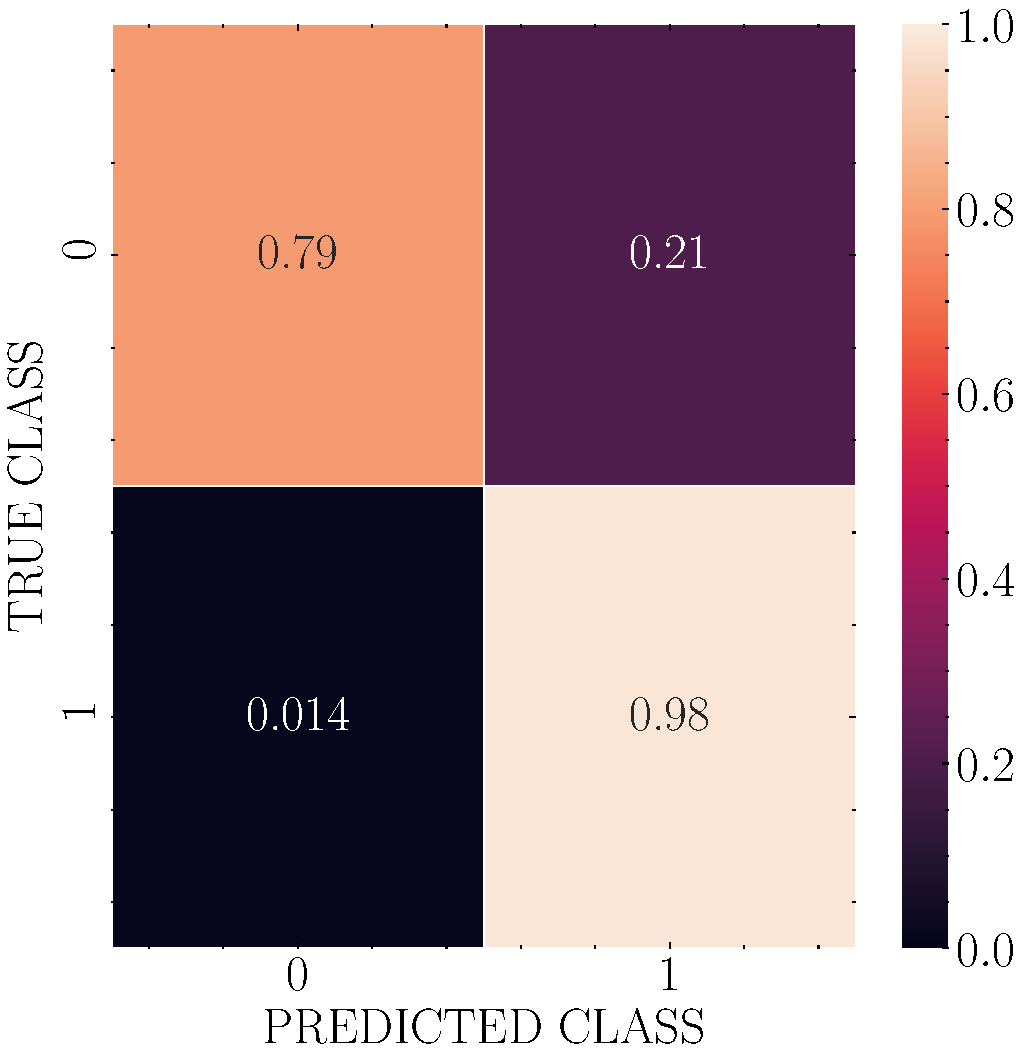
\includegraphics[width=1.5in]{../results/ex1/acc_LS_dataset_Gamma_size_10.pdf}
       \caption{LS, size $10$}
       \label{fig:LS_P1a_10}
    \end{subfigure}
\quad
    \begin{subfigure}[!htbp]{0.2\textwidth}
       \centering
       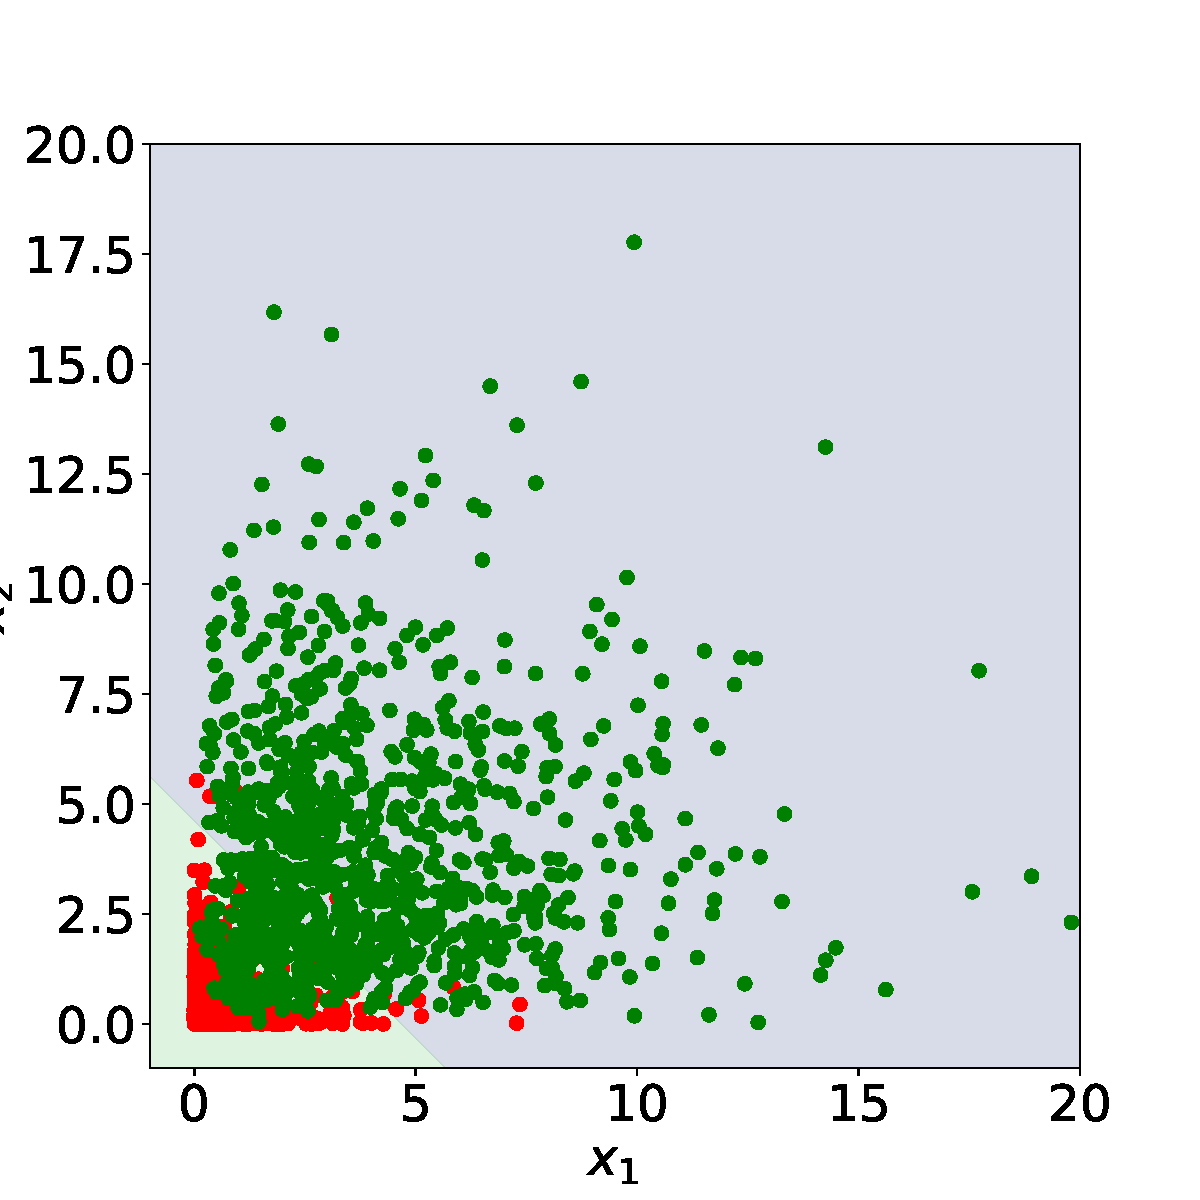
\includegraphics[width=1.5in]{../results/ex1/samples_LS_dataset_Gamma_size_10.pdf}
       \caption{LS Classifier}
       \label{fig:LSD_P1a_10}
    \end{subfigure}
\quad
    \begin{subfigure}[!htbp]{0.2\textwidth}
       \centering
       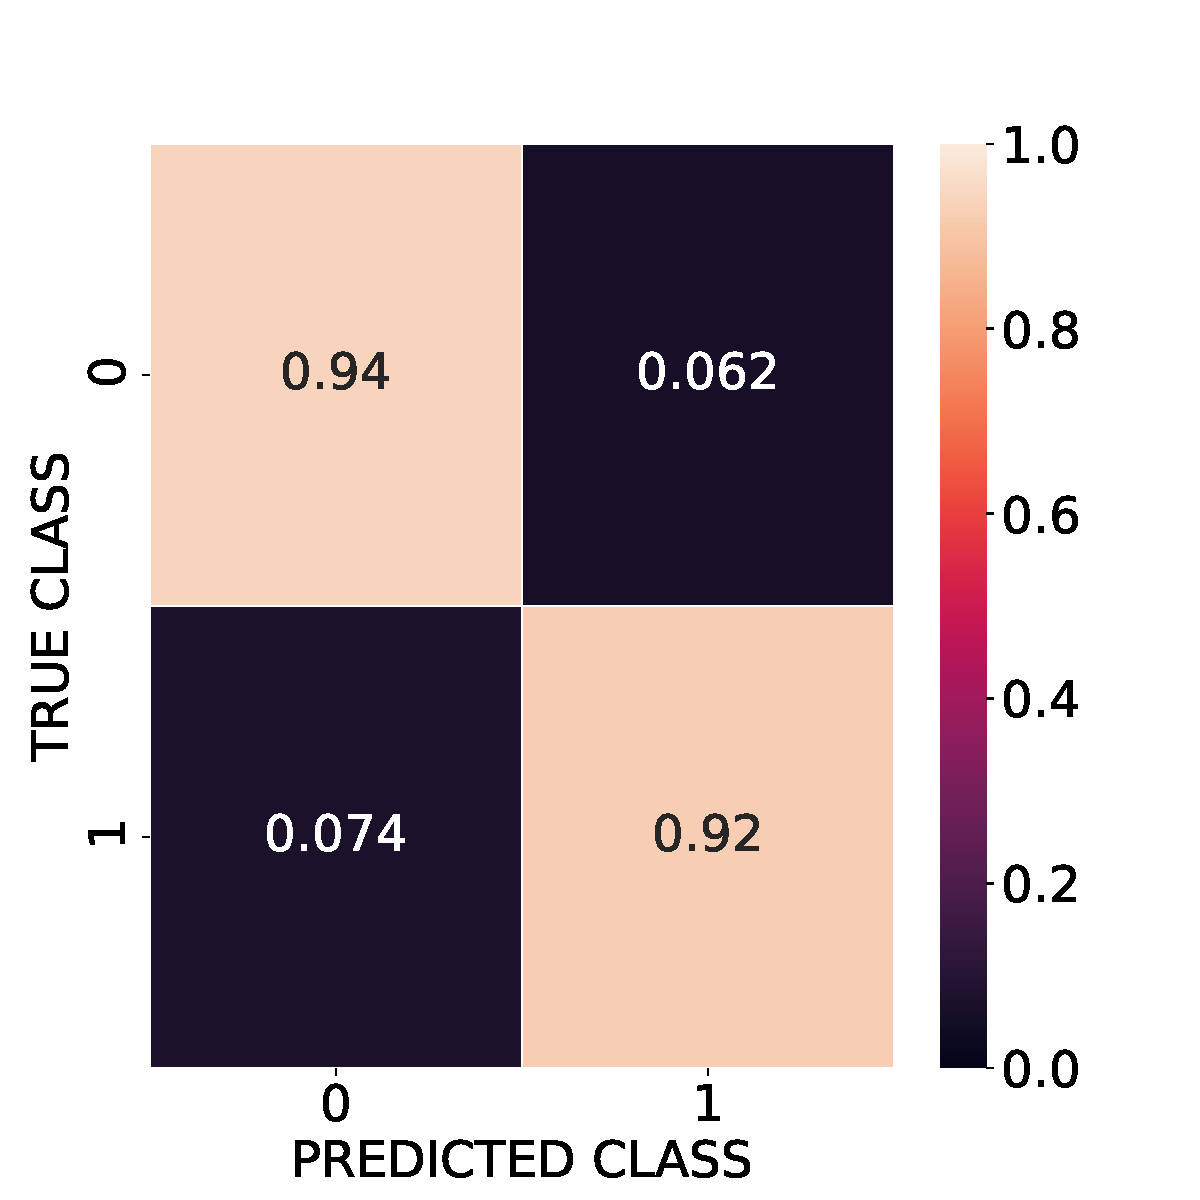
\includegraphics[width=1.5in]{../results/ex1/acc_LOG_dataset_Gamma_size_10.pdf}
       \caption{LOG, size $10$}
       \label{fig:LOG_P1a_10}
    \end{subfigure}
\quad
    \begin{subfigure}[!htbp]{0.2\textwidth}
       \centering
       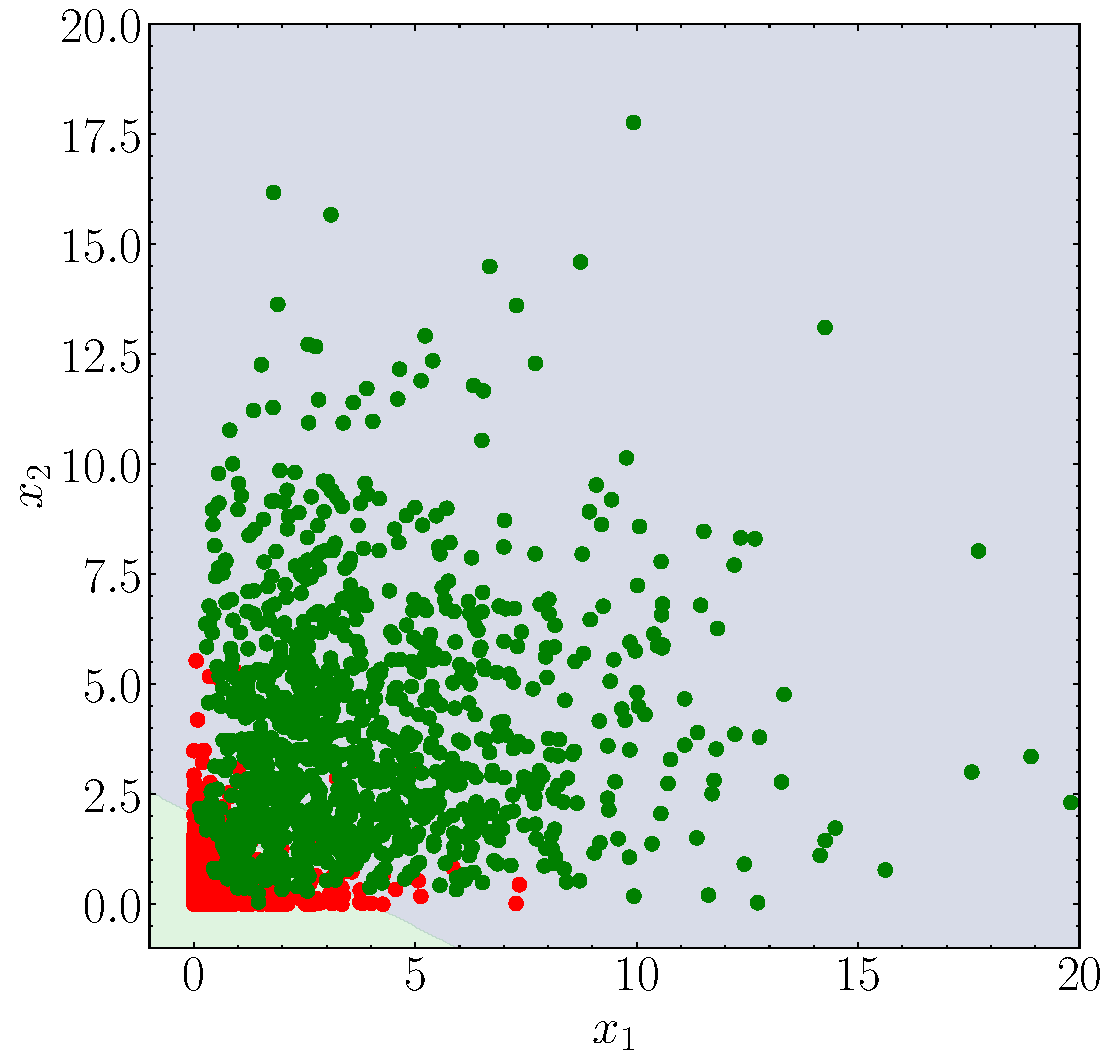
\includegraphics[width=1.5in]{../results/ex1/samples_LOG_dataset_Gamma_size_10.pdf}
       \caption{LOG Classifier}
       \label{fig:LOGD_P1a_10}
    \end{subfigure}
    
    \begin{subfigure}[!htbp]{0.2\textwidth}
       \centering
       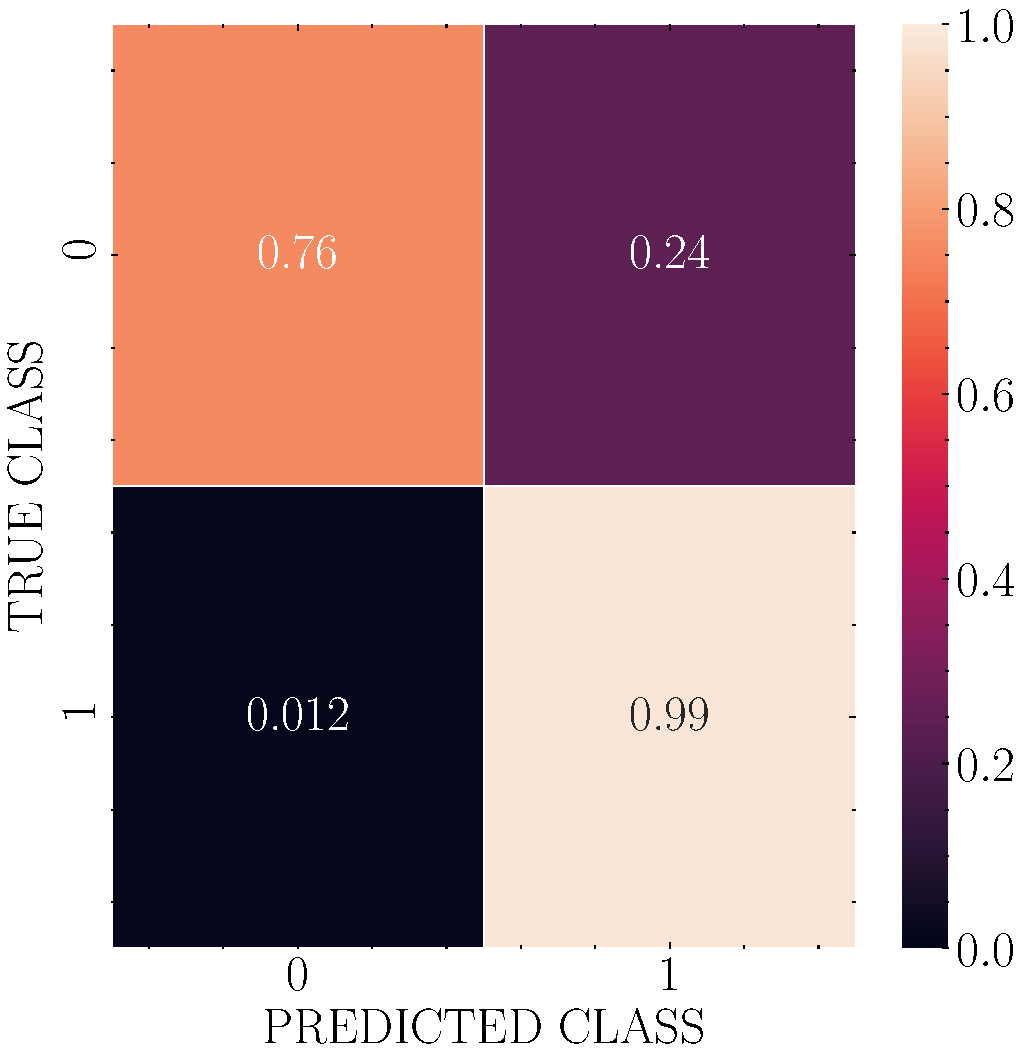
\includegraphics[width=1.5in]{../results/ex1/acc_LS_dataset_Gamma_size_50.pdf}
       \caption{LS, size $50$}
       \label{fig:LS_P1a_50}
    \end{subfigure}
\quad
    \begin{subfigure}[!htbp]{0.2\textwidth}
       \centering
       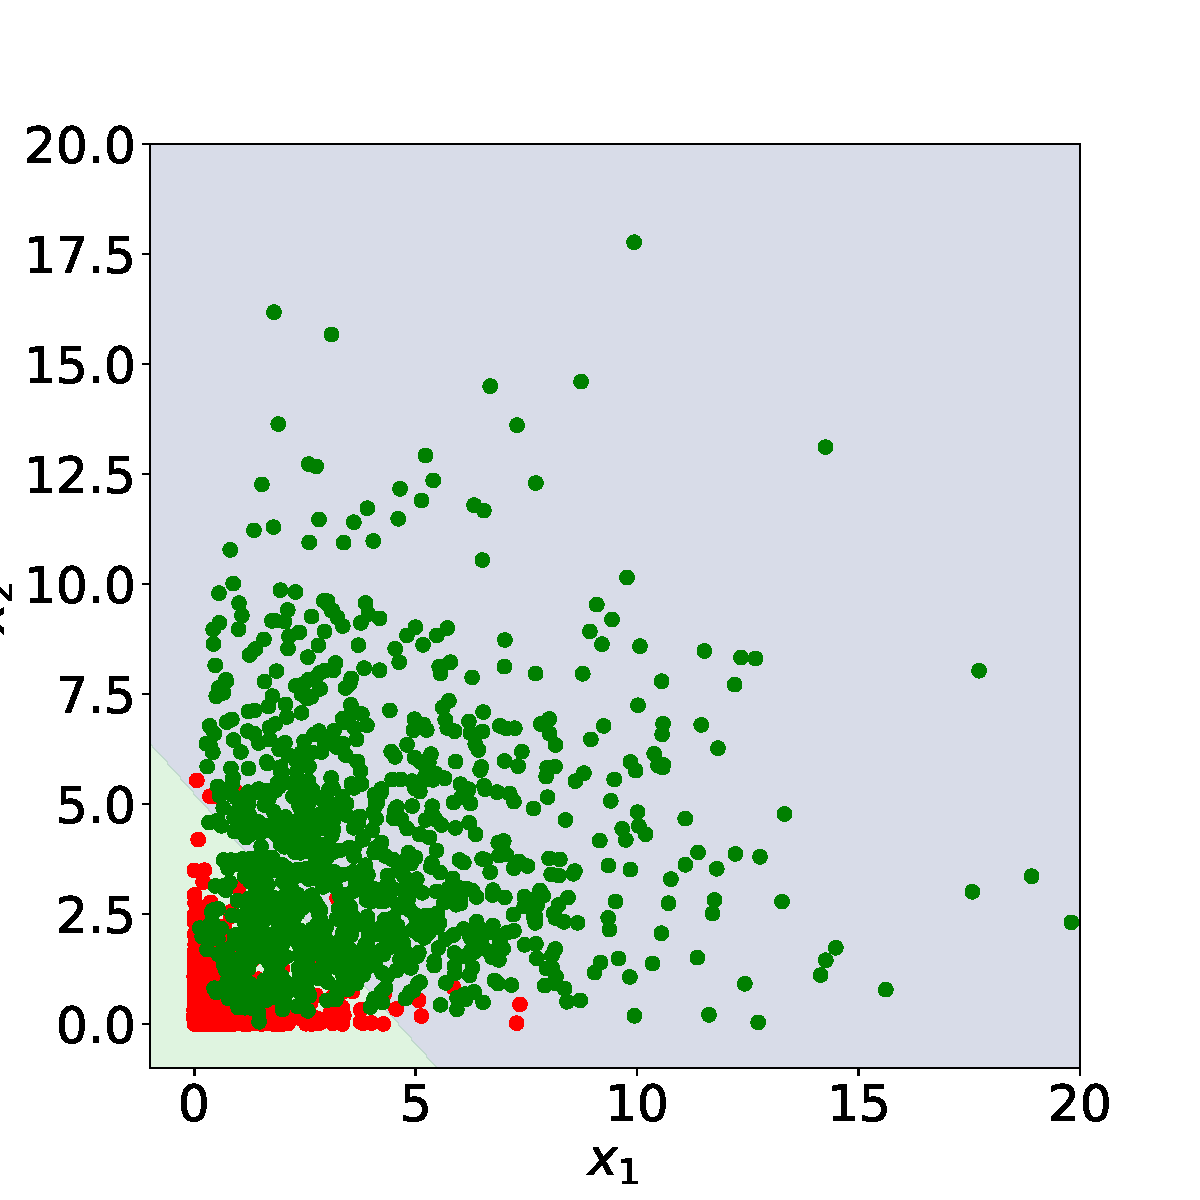
\includegraphics[width=1.5in]{../results/ex1/samples_LS_dataset_Gamma_size_50.pdf}
       \caption{LS Classifier}
       \label{fig:LSD_P1a_50}
    \end{subfigure}
\quad
    \begin{subfigure}[!htbp]{0.2\textwidth}
       \centering
       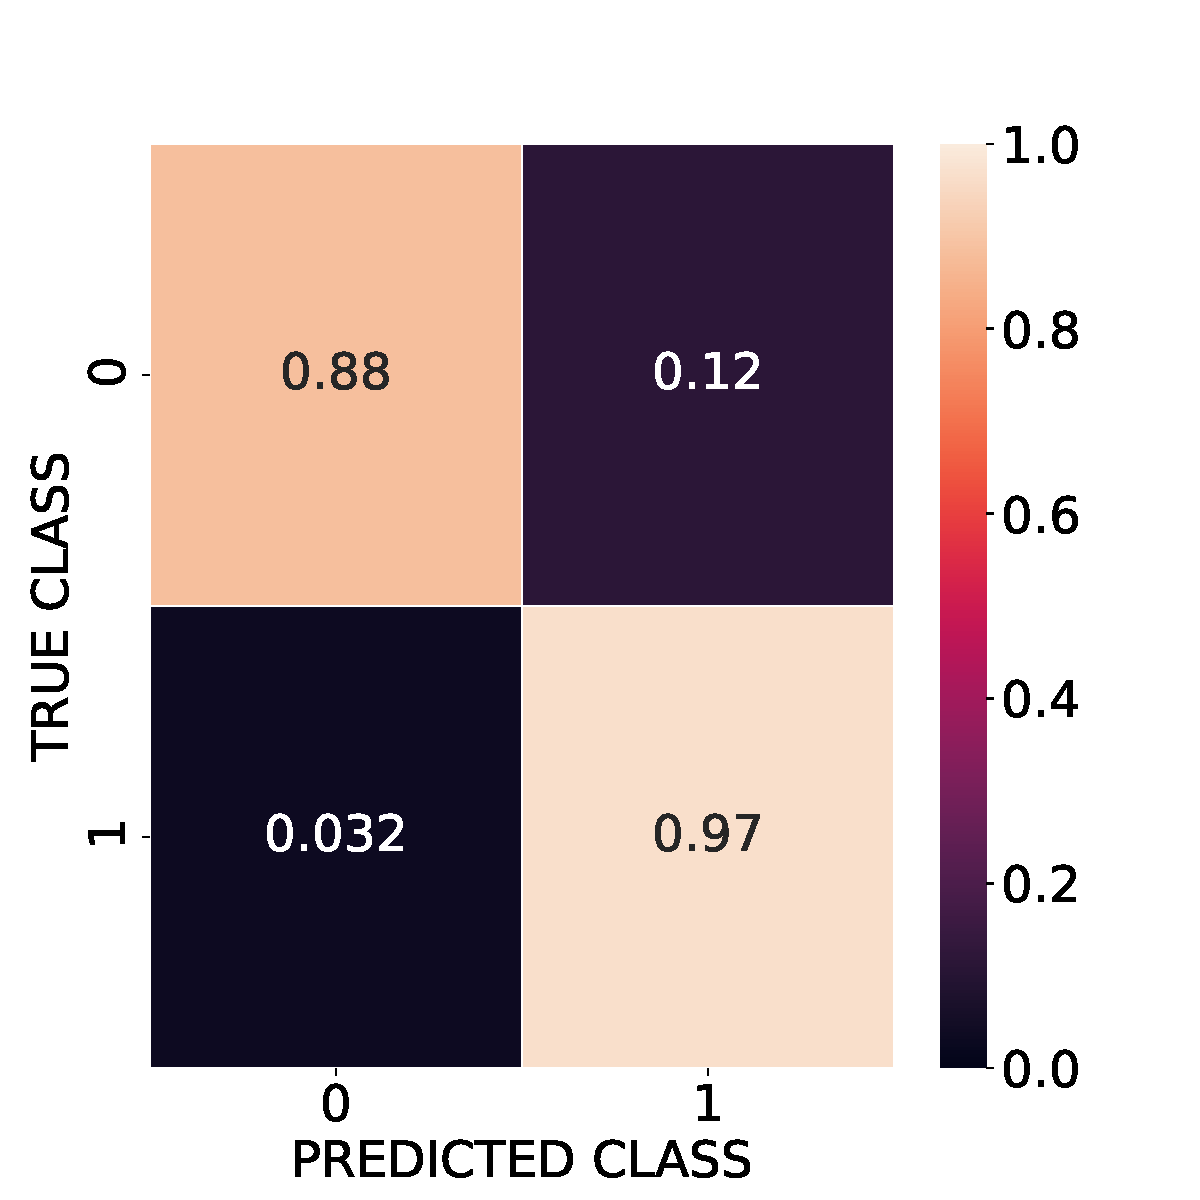
\includegraphics[width=1.5in]{../results/ex1/acc_LOG_dataset_Gamma_size_50.pdf}
       \caption{LOG, size $50$}
       \label{fig:LOG_P1a_50}
    \end{subfigure}
\quad
    \begin{subfigure}[!htbp]{0.2\textwidth}
       \centering
       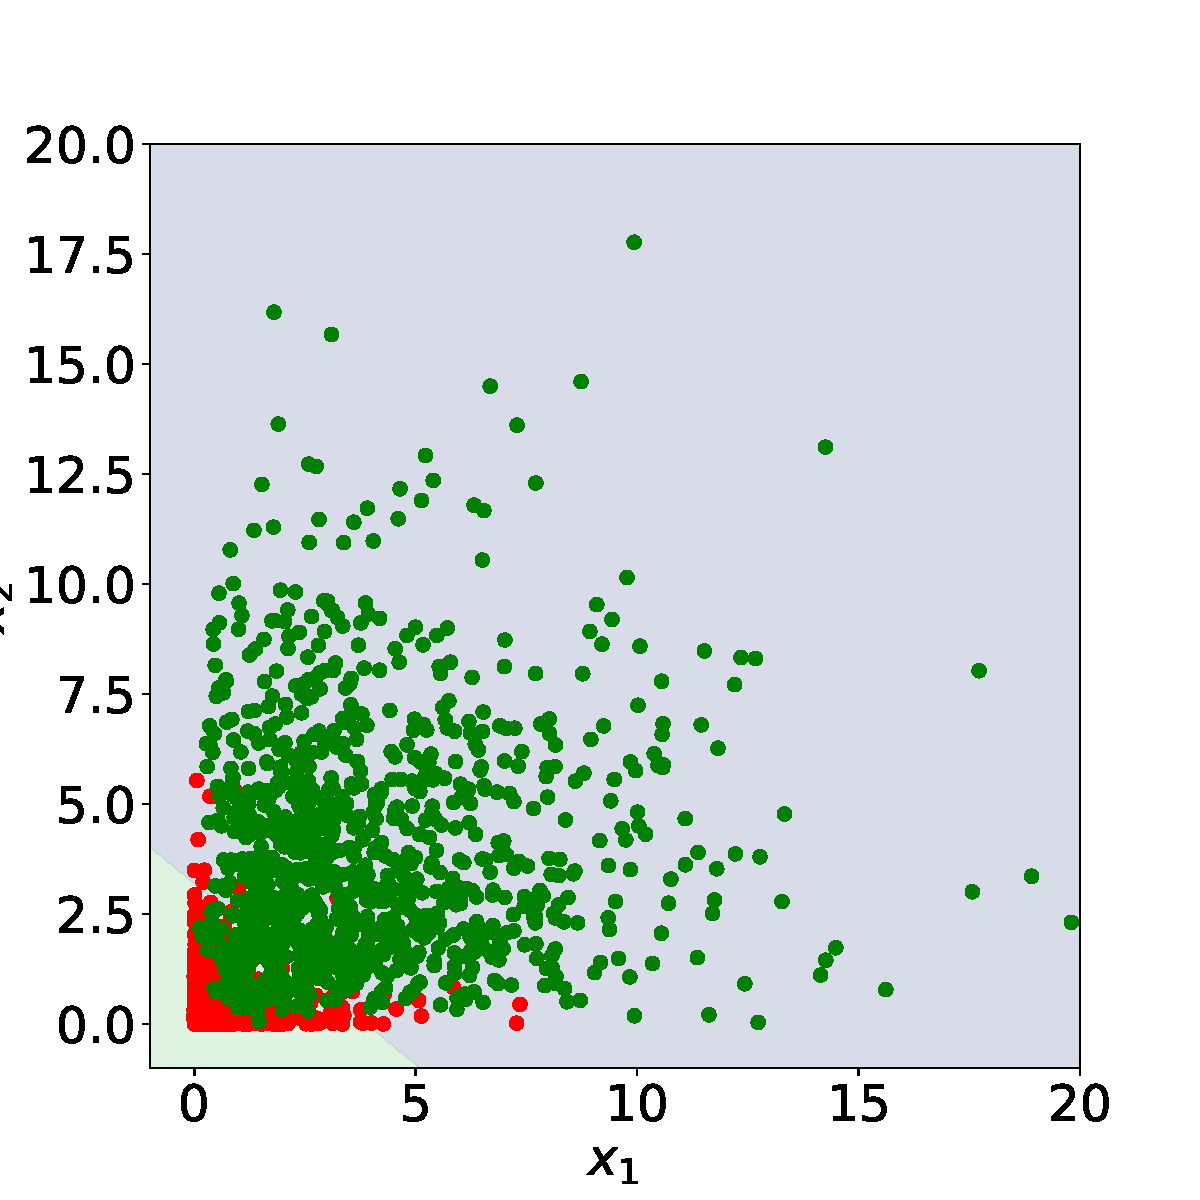
\includegraphics[width=1.5in]{../results/ex1/samples_LOG_dataset_Gamma_size_50.pdf}
       \caption{LOG Classifier}
       \label{fig:LOGD_P1a_50}
    \end{subfigure}
    
    \begin{subfigure}[!htbp]{0.2\textwidth}
       \centering
       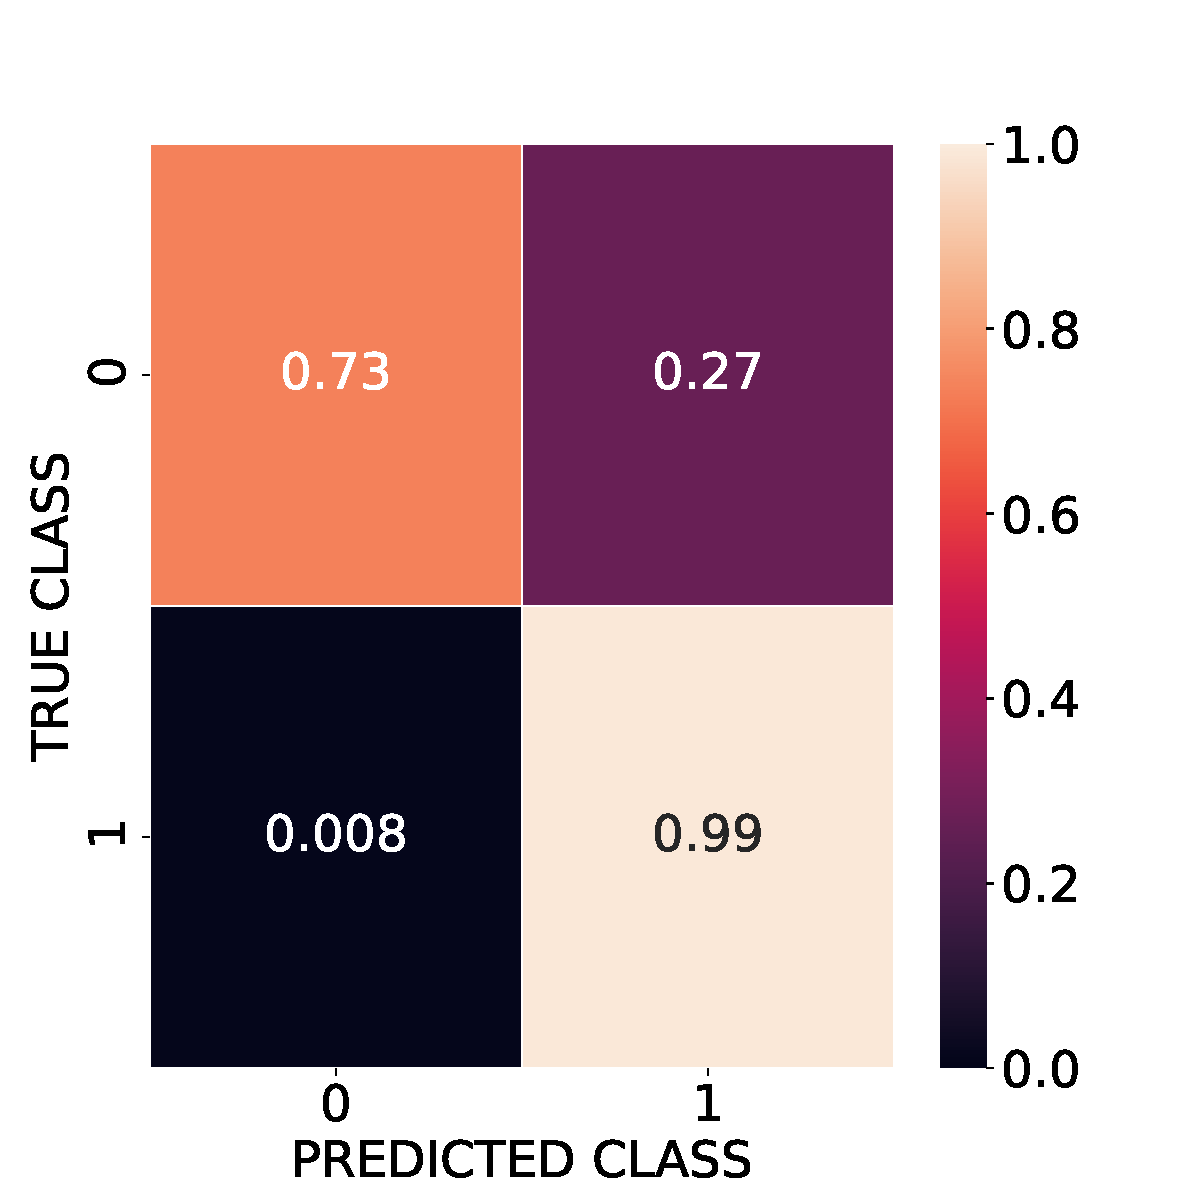
\includegraphics[width=1.5in]{../results/ex1/acc_LS_dataset_Gamma_size_100.pdf}
       \caption{LS, size $100$}
       \label{fig:LS_P1a_100}
    \end{subfigure}
\quad
    \begin{subfigure}[!htbp]{0.2\textwidth}
       \centering
       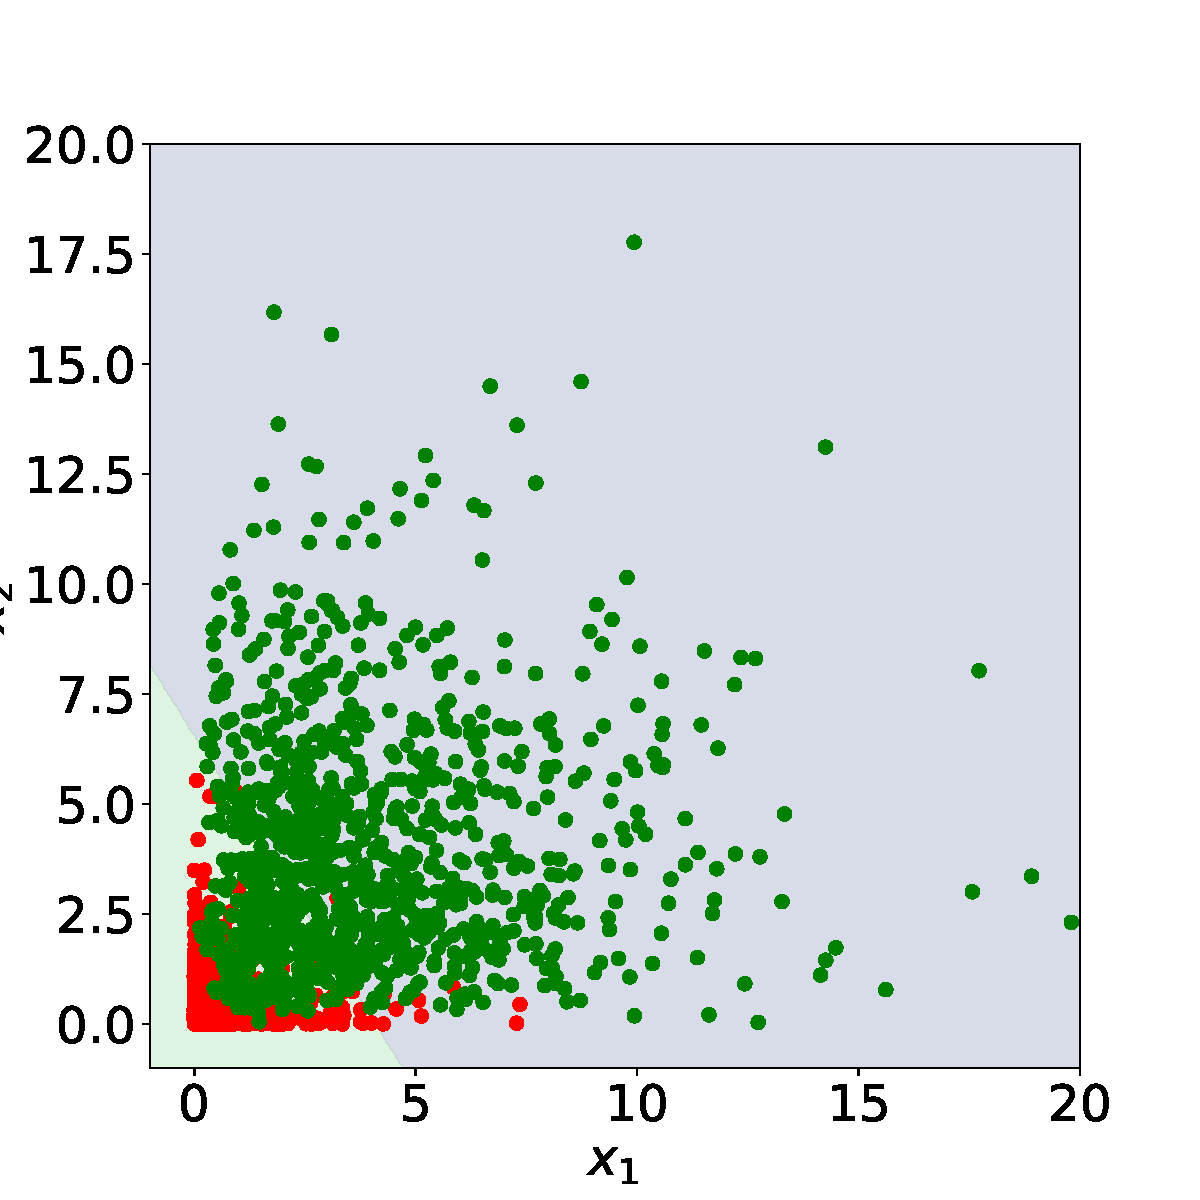
\includegraphics[width=1.5in]{../results/ex1/samples_LS_dataset_Gamma_size_100.pdf}
       \caption{LS Classifier}
       \label{fig:LSD_P1a_100}
    \end{subfigure}
\quad
    \begin{subfigure}[!htbp]{0.2\textwidth}
       \centering
       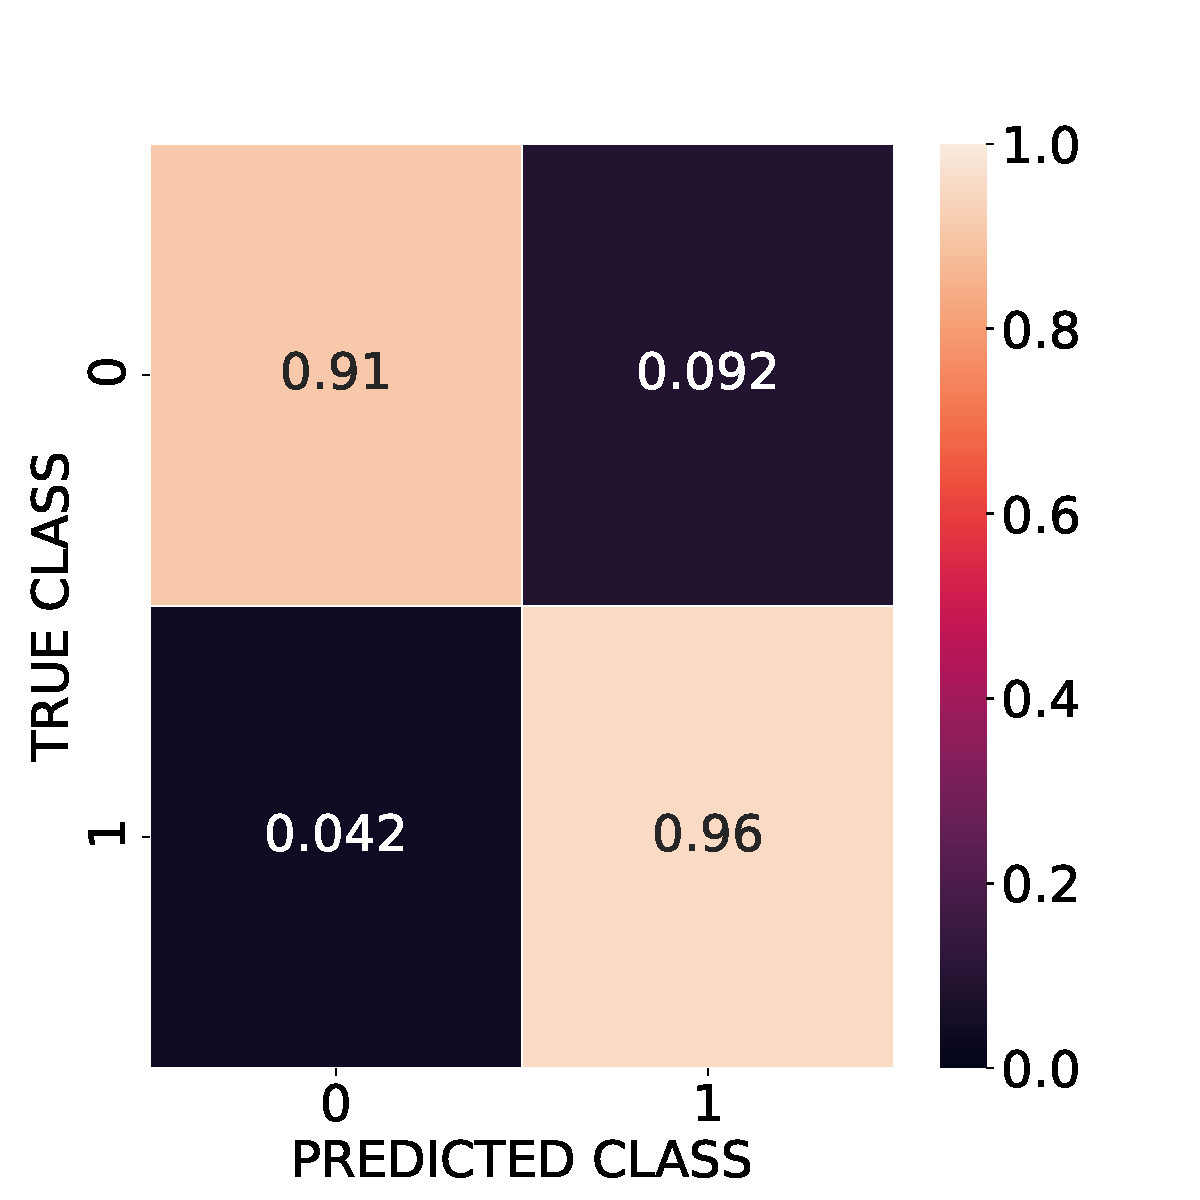
\includegraphics[width=1.5in]{../results/ex1/acc_LOG_dataset_Gamma_size_100.pdf}
       \caption{LOG, size $100$}
       \label{fig:LOG_P1a_100}
    \end{subfigure}
\quad
    \begin{subfigure}[!htbp]{0.2\textwidth}
       \centering
       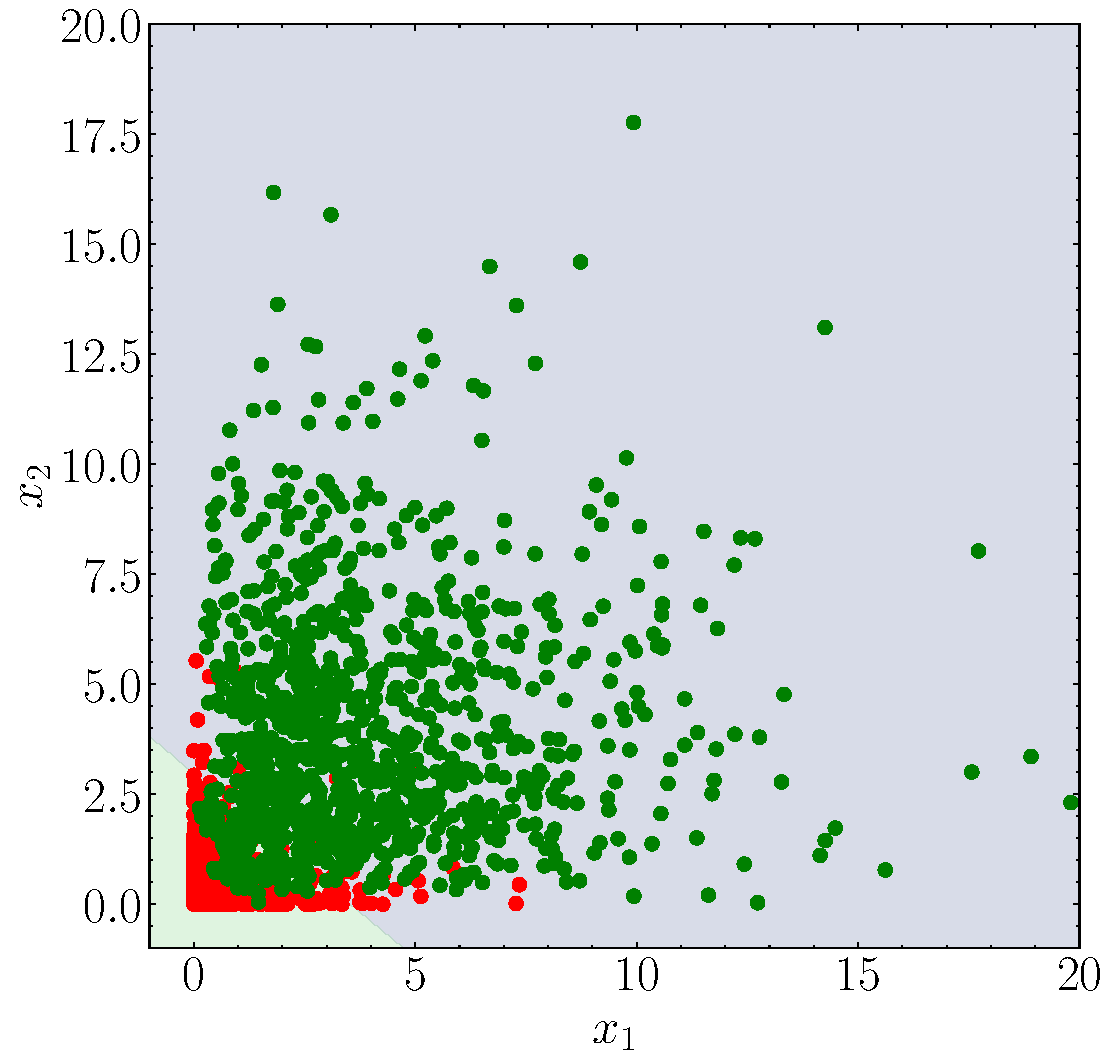
\includegraphics[width=1.5in]{../results/ex1/samples_LOG_dataset_Gamma_size_100.pdf}
       \caption{LOG Classifier}
       \label{fig:LOGD_P1a_100}
    \end{subfigure} 
    
    \begin{subfigure}[!htbp]{0.2\textwidth}
       \centering
       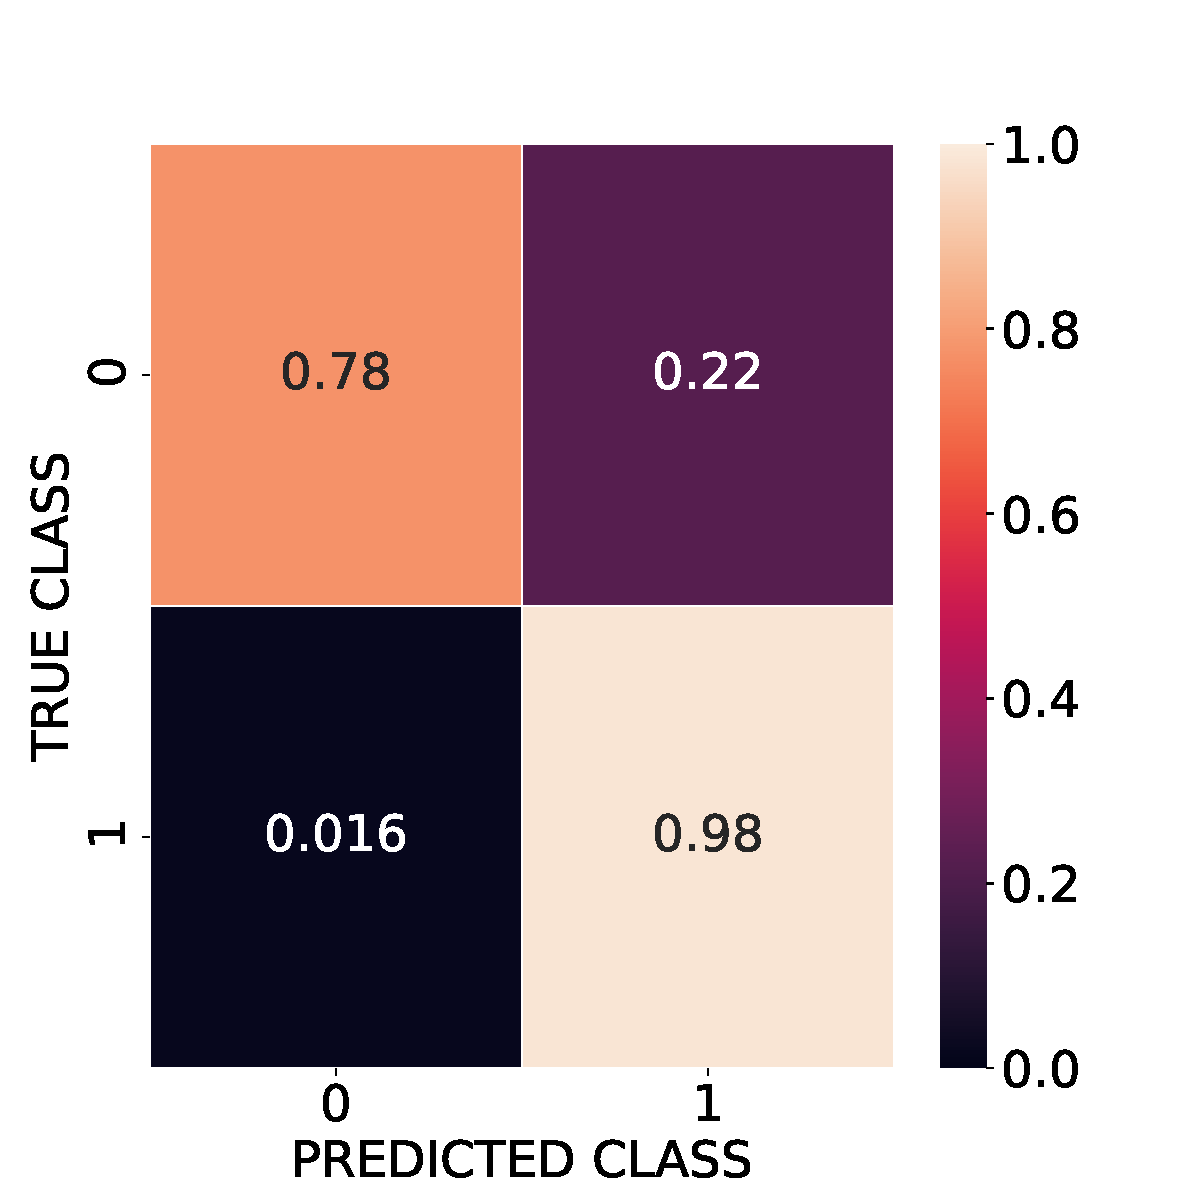
\includegraphics[width=1.5in]{../results/ex1/acc_LS_dataset_Gamma_size_500.pdf}
       \caption{LS, size $500$}
       \label{fig:LS_P1a_500}
    \end{subfigure}
\quad
    \begin{subfigure}[!htbp]{0.2\textwidth}
       \centering
       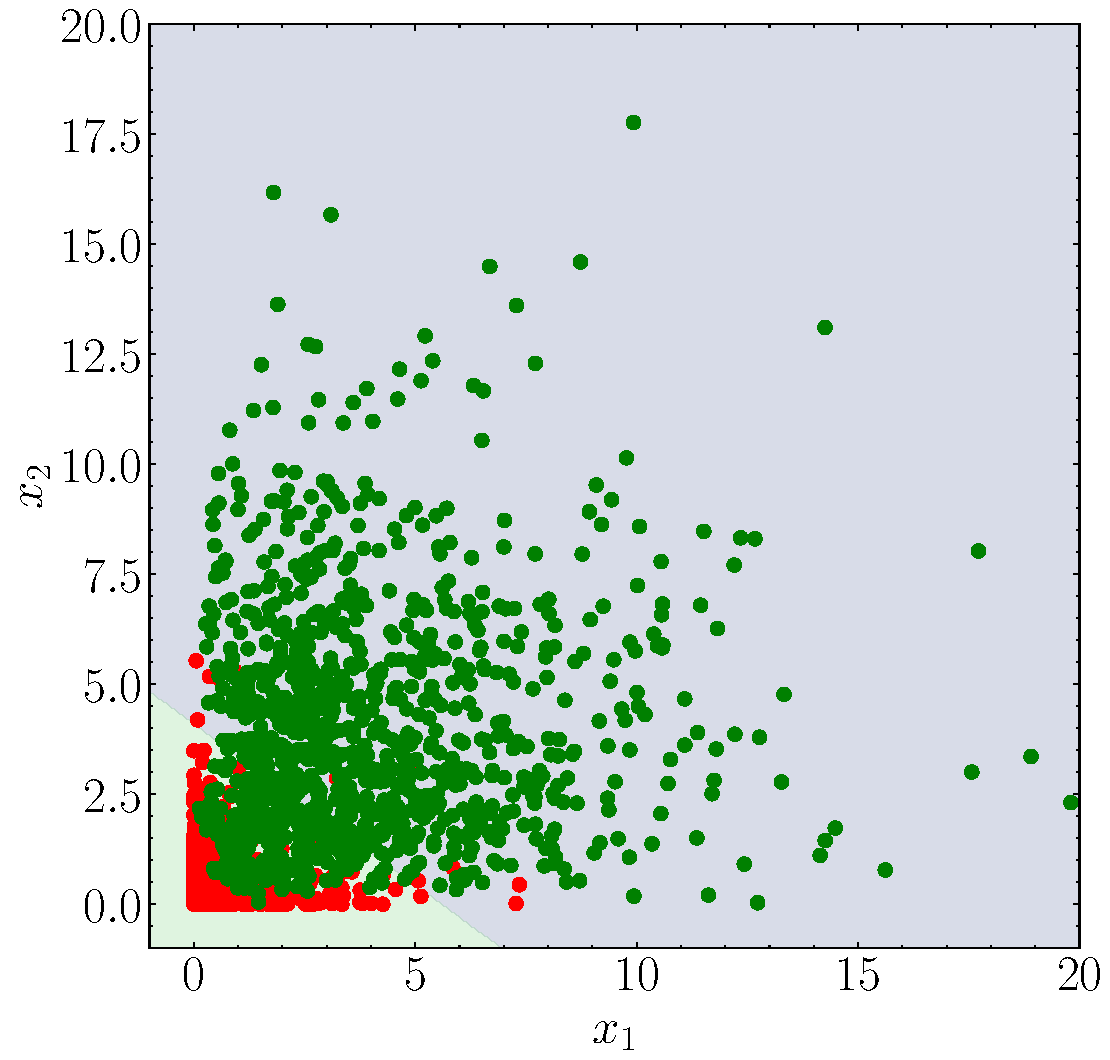
\includegraphics[width=1.5in]{../results/ex1/samples_LS_dataset_Gamma_size_500.pdf}
       \caption{LS Classifier}
       \label{fig:LSD_P1a_500}
    \end{subfigure}
\quad
    \begin{subfigure}[!htbp]{0.2\textwidth}
       \centering
       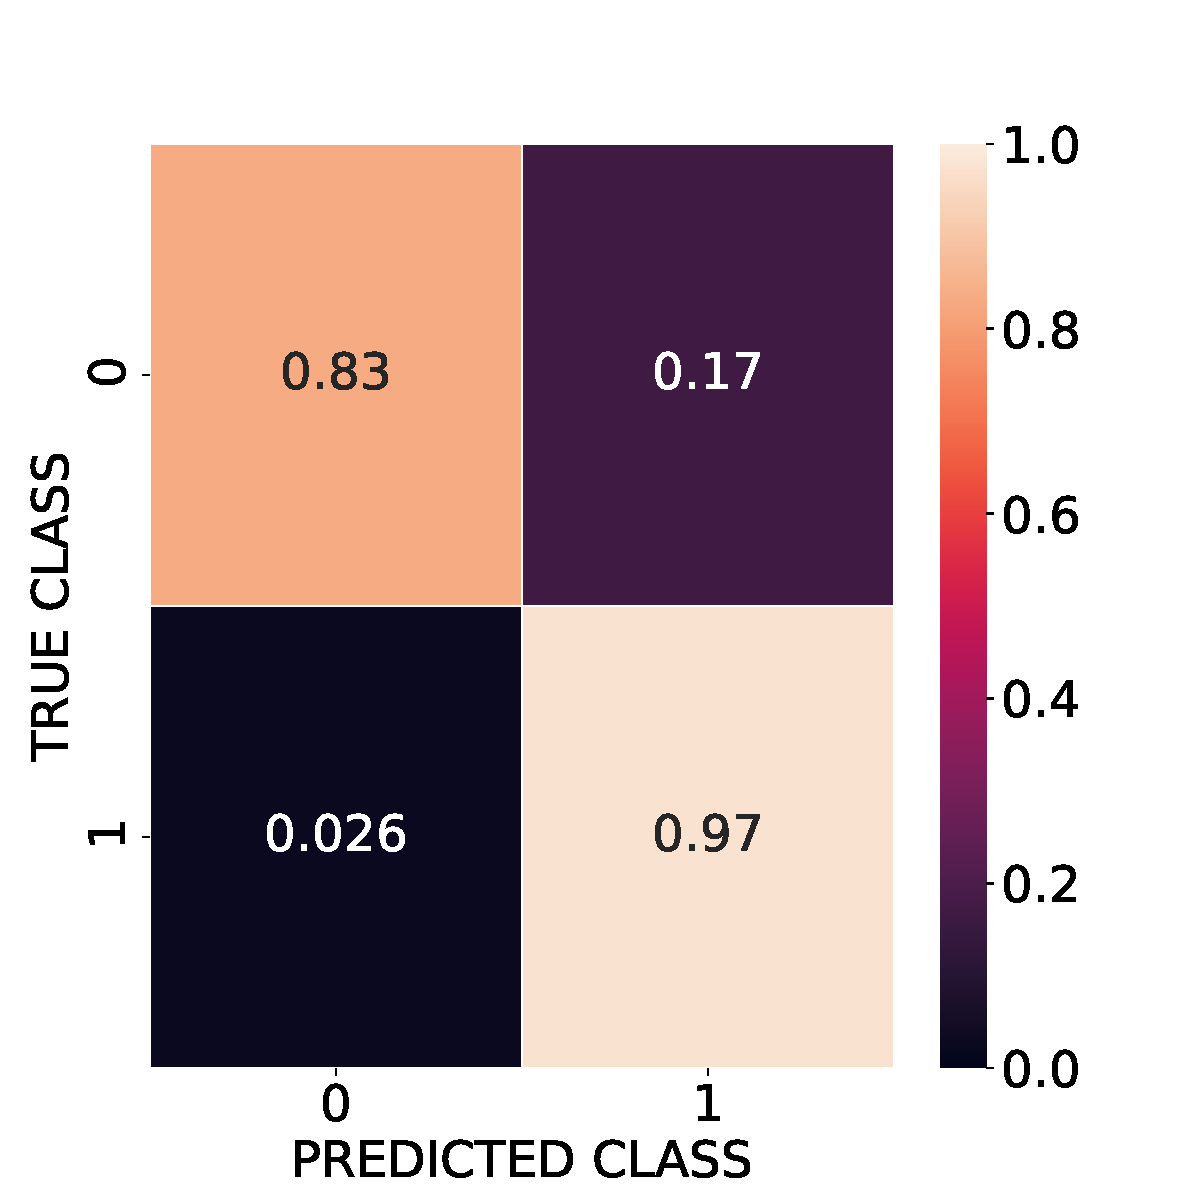
\includegraphics[width=1.5in]{../results/ex1/acc_LOG_dataset_Gamma_size_500.pdf}
       \caption{LOG, size $500$}
       \label{fig:LOG_P1a_500}
    \end{subfigure}
\quad
    \begin{subfigure}[!htbp]{0.2\textwidth}
       \centering
       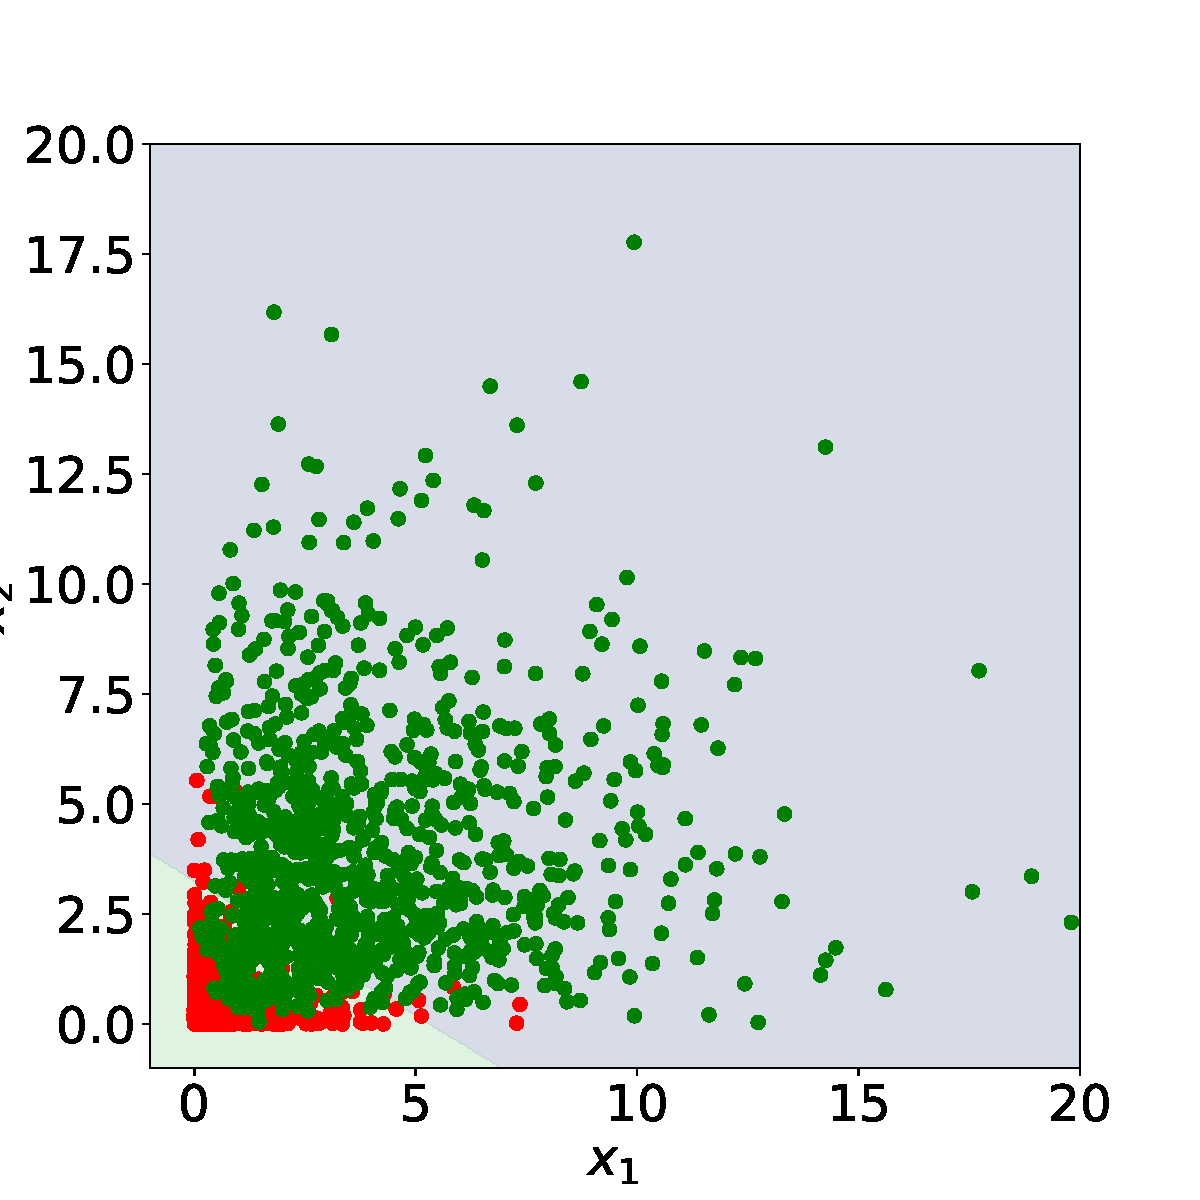
\includegraphics[width=1.5in]{../results/ex1/samples_LOG_dataset_Gamma_size_500.pdf}
       \caption{LOG Classifier}
       \label{fig:LOGD_P1a_500}
    \end{subfigure} 
    
    \begin{subfigure}[!htbp]{0.2\textwidth}
       \centering
       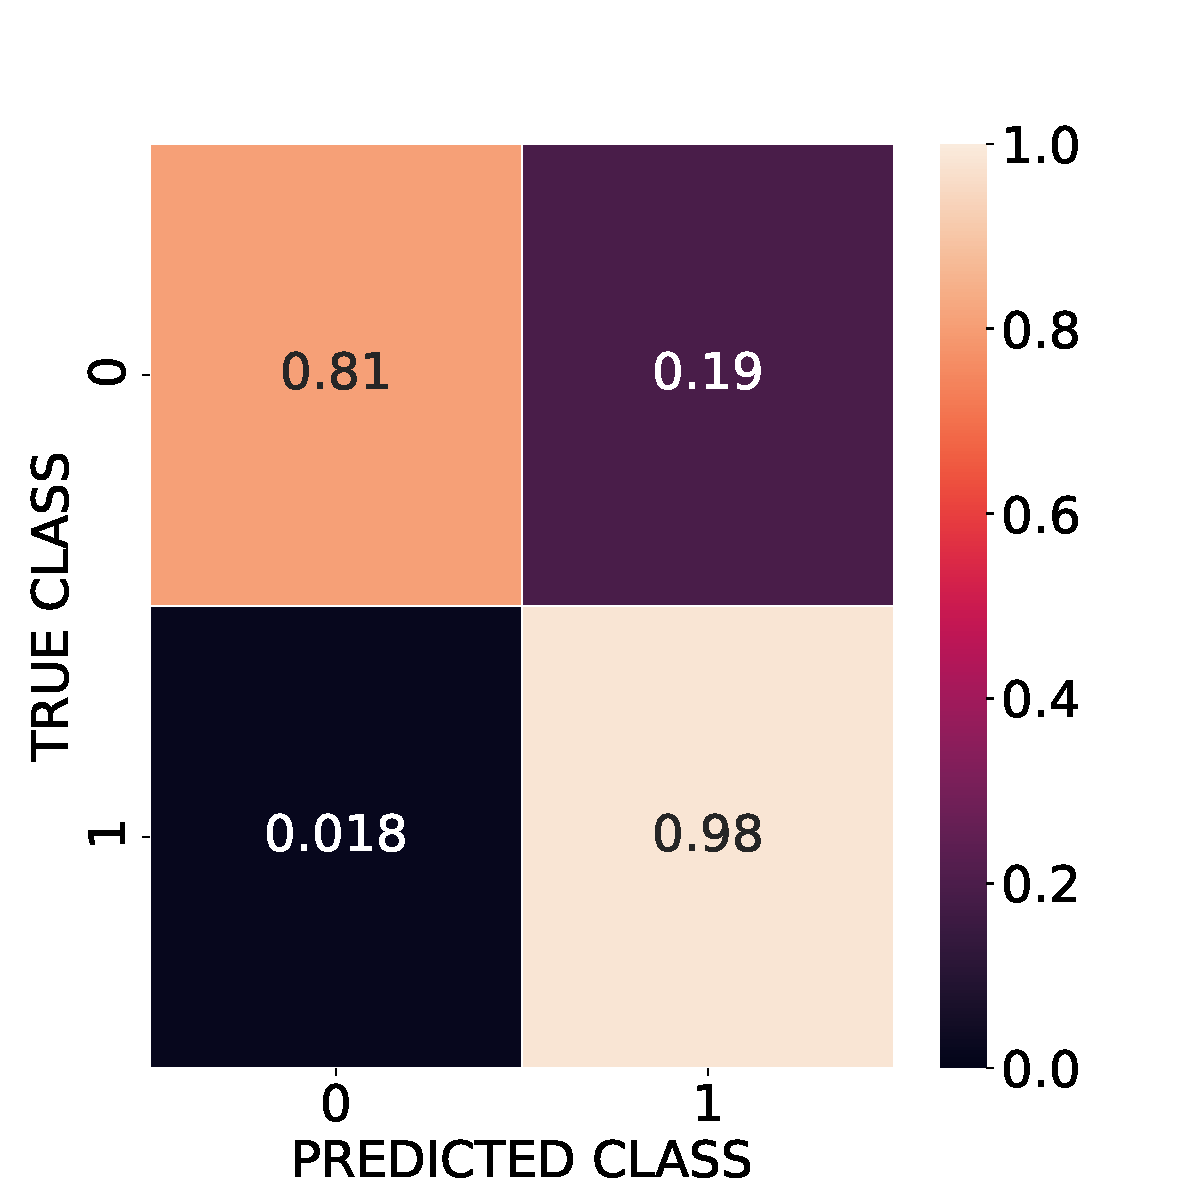
\includegraphics[width=1.5in]{../results/ex1/acc_LS_dataset_Gamma_size_999.pdf}
       \caption{LS, size $999$}
       \label{fig:LS_P1a_999}
    \end{subfigure}
\quad
    \begin{subfigure}[!htbp]{0.2\textwidth}
       \centering
       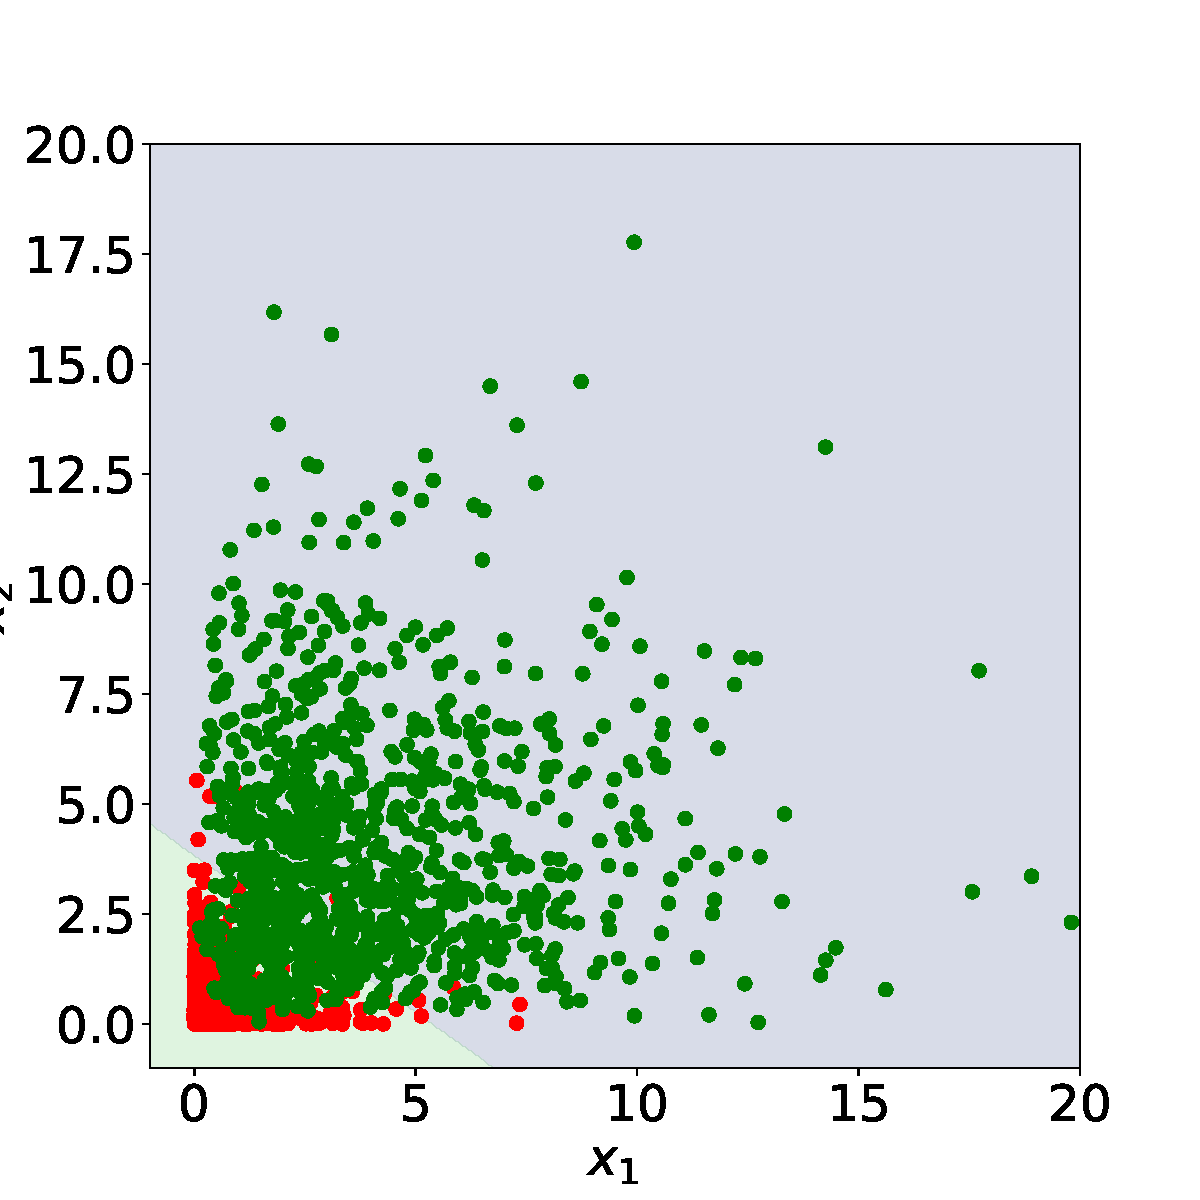
\includegraphics[width=1.5in]{../results/ex1/samples_LS_dataset_Gamma_size_999.pdf}
       \caption{LS Classifier}
       \label{fig:LSD_P1a_999}
    \end{subfigure}
\quad
    \begin{subfigure}[!htbp]{0.2\textwidth}
       \centering
       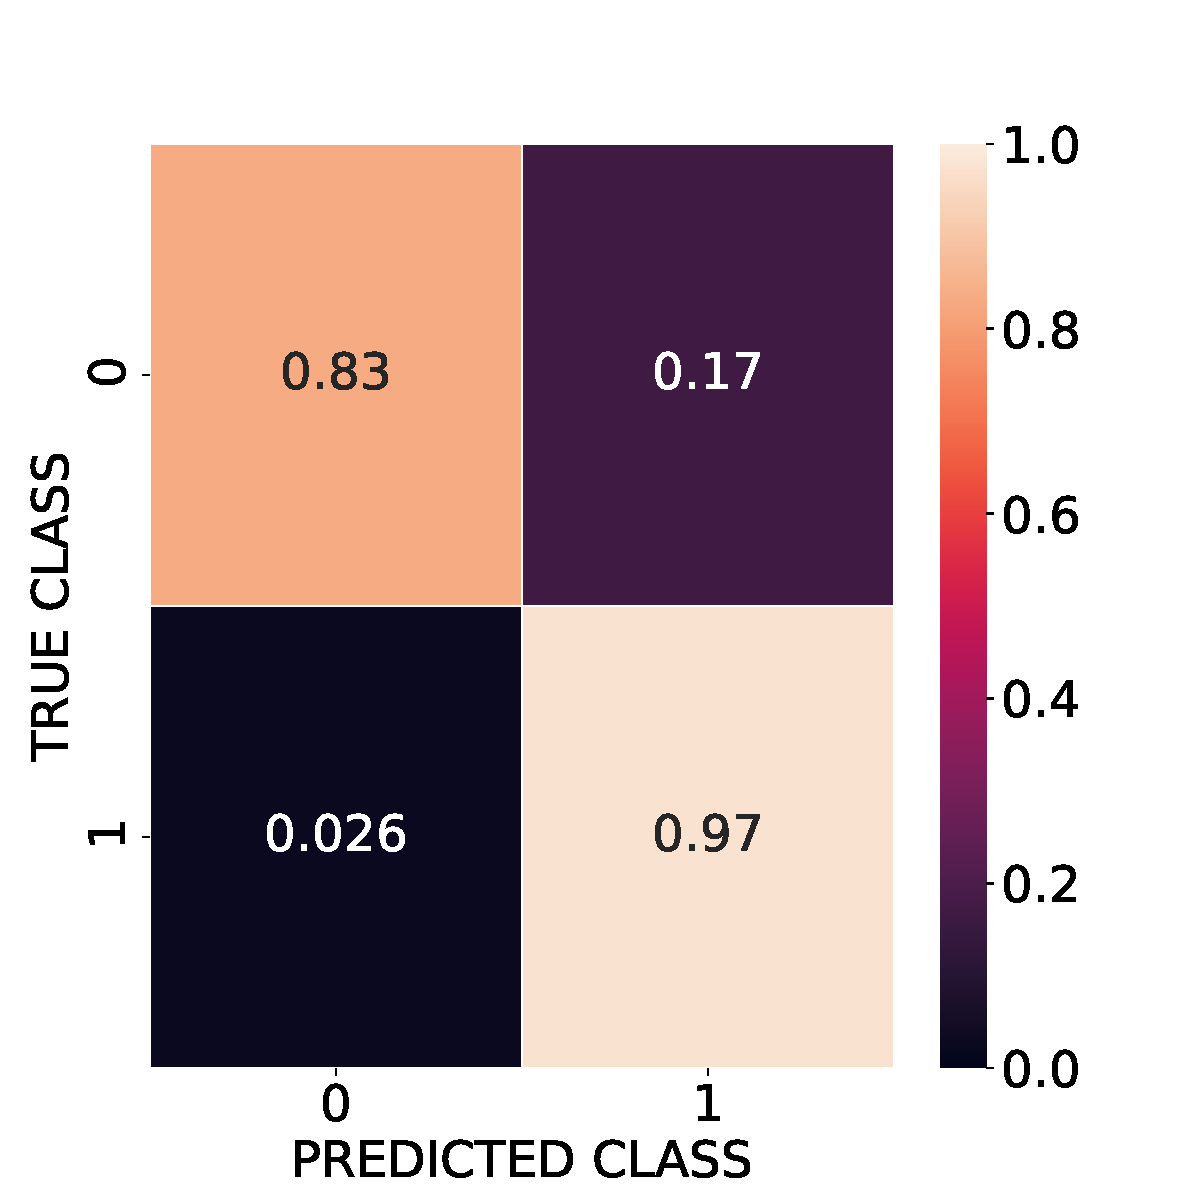
\includegraphics[width=1.5in]{../results/ex1/acc_LOG_dataset_Gamma_size_999.pdf}
       \caption{LOG, size $999$}
       \label{fig:LOG_P1a_999}
    \end{subfigure}
\quad
    \begin{subfigure}[!htbp]{0.2\textwidth}
       \centering
       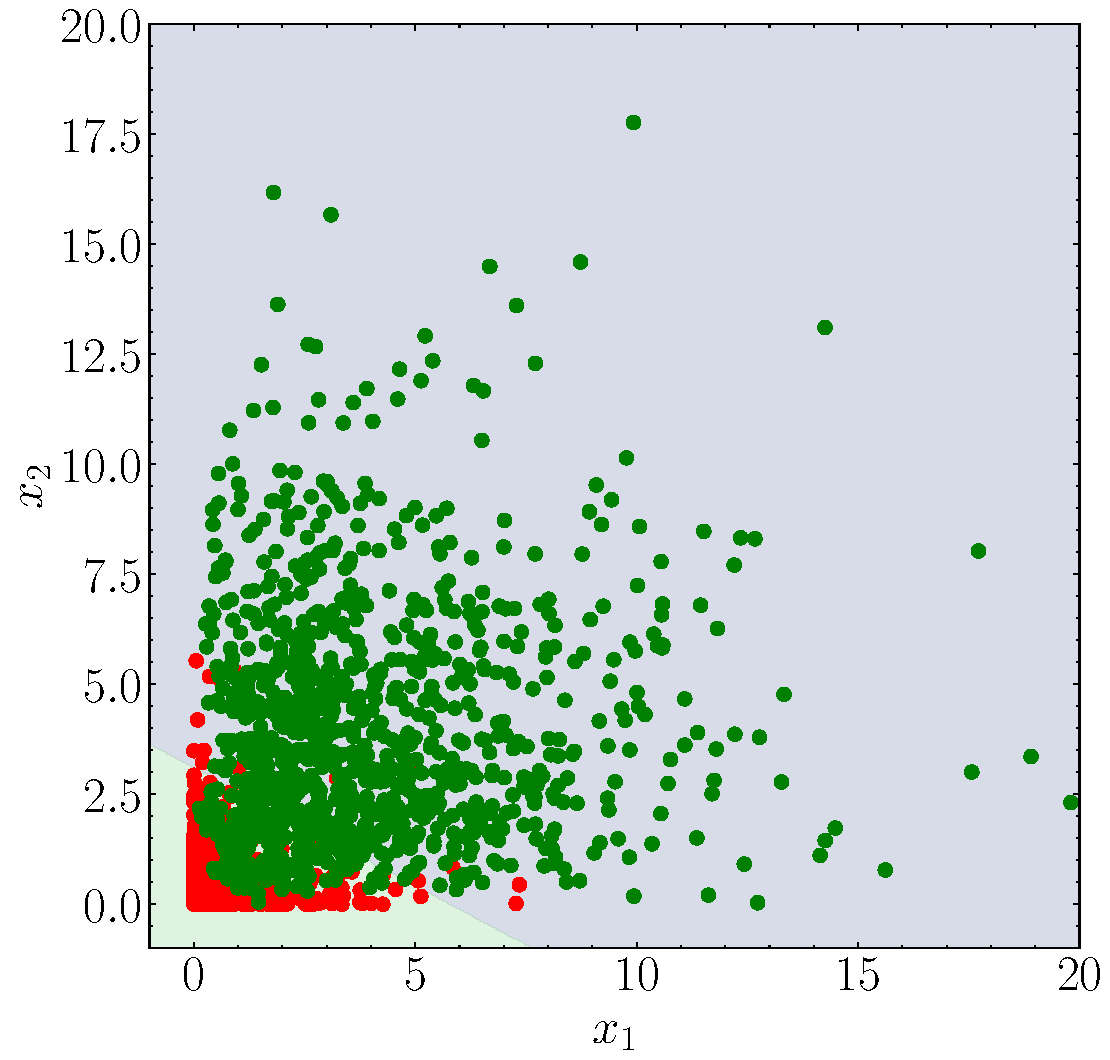
\includegraphics[width=1.5in]{../results/ex1/samples_LOG_dataset_Gamma_size_999.pdf}
       \caption{LOG Classifier}
       \label{fig:LOGD_P1a_999}
    \end{subfigure}     

\caption{Linear Least-Squares Classification and Logistic Regression.}
\label{fig:ex1_P1a}
\end{figure}

% ------------------------------------------------------------------------------------------------------------------------------------------------------

\problem{Problem (1.b) Uniform-distributed Classes in 2D}
\label{prob:1.b}

\begin{figure}[!htbp]
\centering
    \begin{subfigure}[!htbp]{0.2\textwidth}
       \centering
       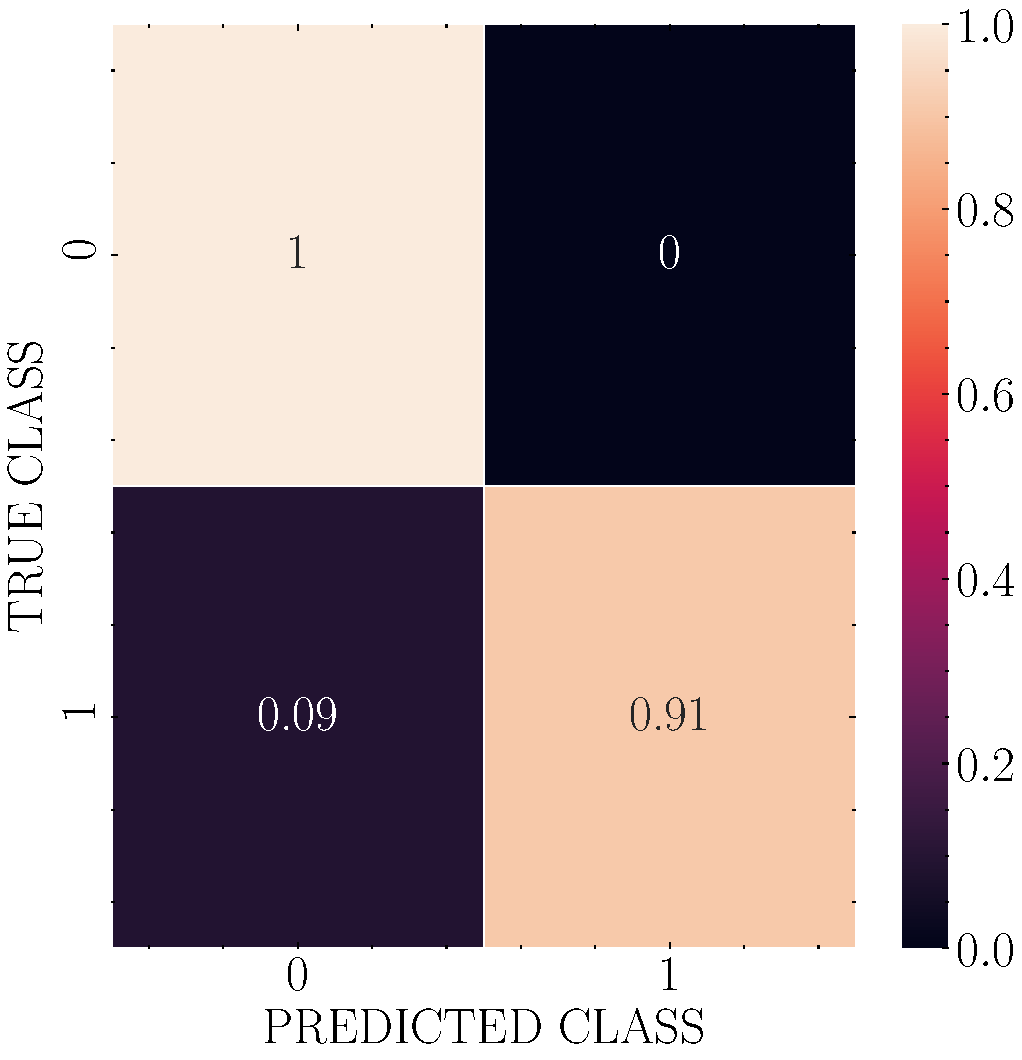
\includegraphics[width=1.5in]{../results/ex1/acc_LS_dataset_Uniform_size_10.pdf}
       \caption{LS, size $10$}
       \label{fig:LS_P1a_10}
    \end{subfigure}
\quad
    \begin{subfigure}[!htbp]{0.2\textwidth}
       \centering
       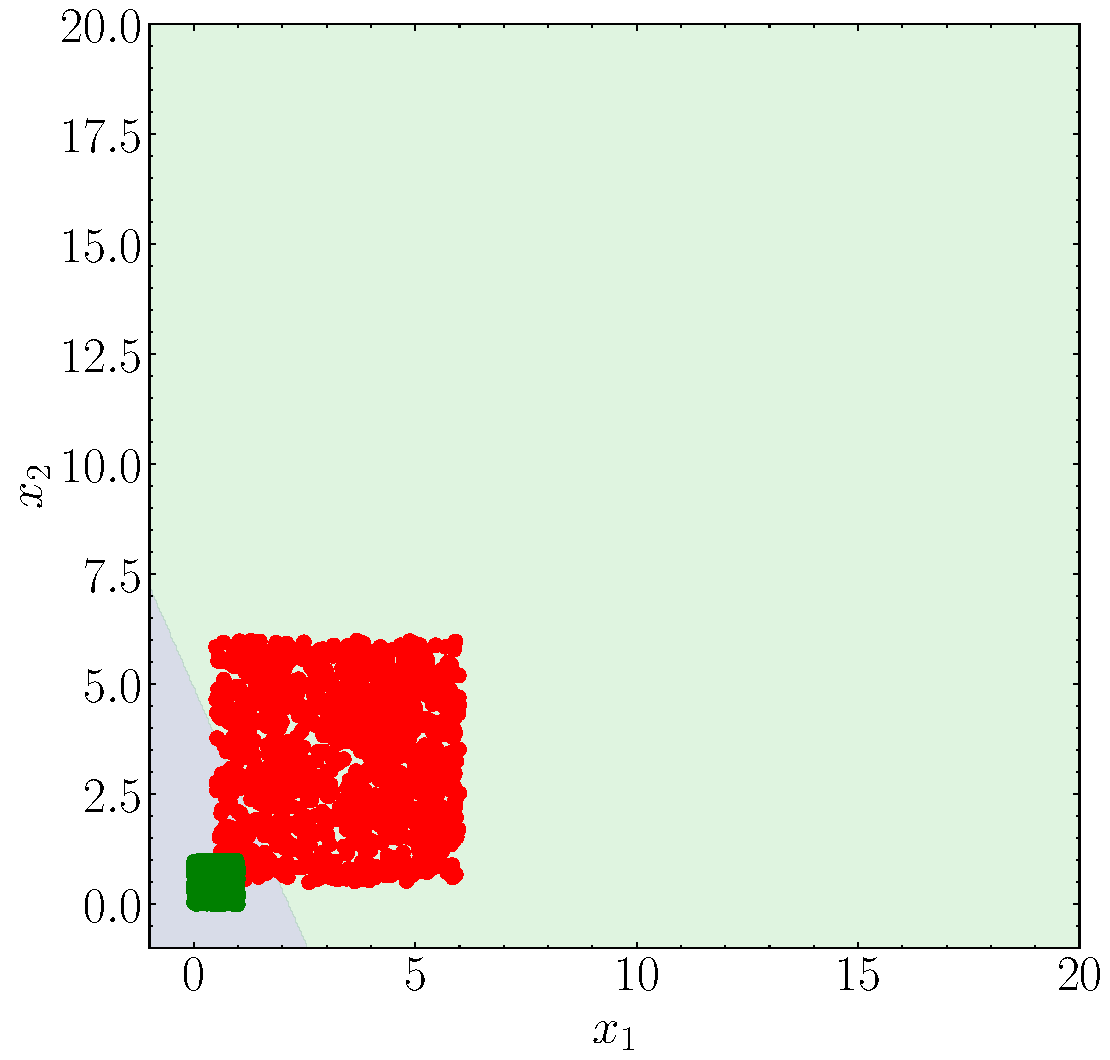
\includegraphics[width=1.5in]{../results/ex1/samples_LS_dataset_Uniform_size_10.pdf}
       \caption{LS Classifier}
       \label{fig:LSD_P1a_10}
    \end{subfigure}
\quad
    \begin{subfigure}[!htbp]{0.2\textwidth}
       \centering
       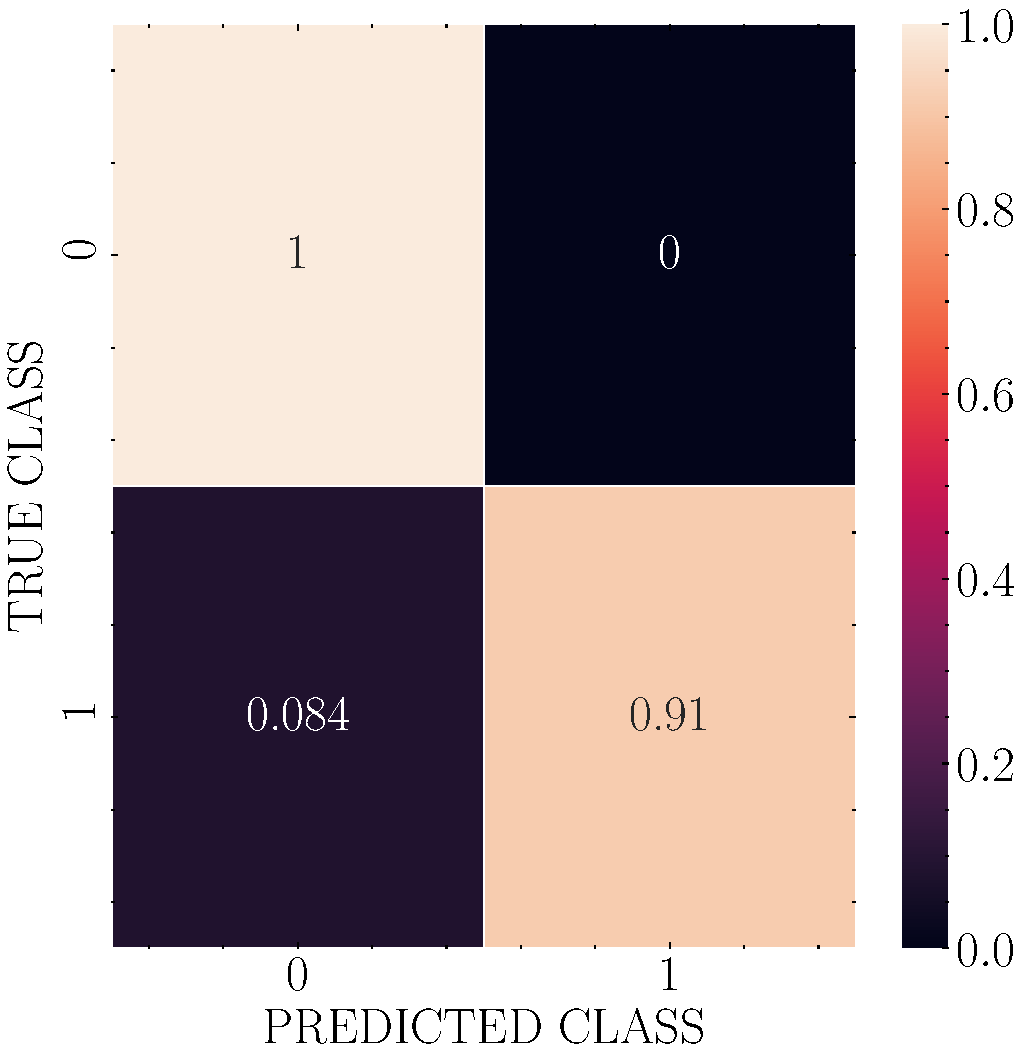
\includegraphics[width=1.5in]{../results/ex1/acc_LOG_dataset_Uniform_size_10.pdf}
       \caption{LOG, size $10$}
       \label{fig:LOG_P1a_10}
    \end{subfigure}
\quad
    \begin{subfigure}[!htbp]{0.2\textwidth}
       \centering
       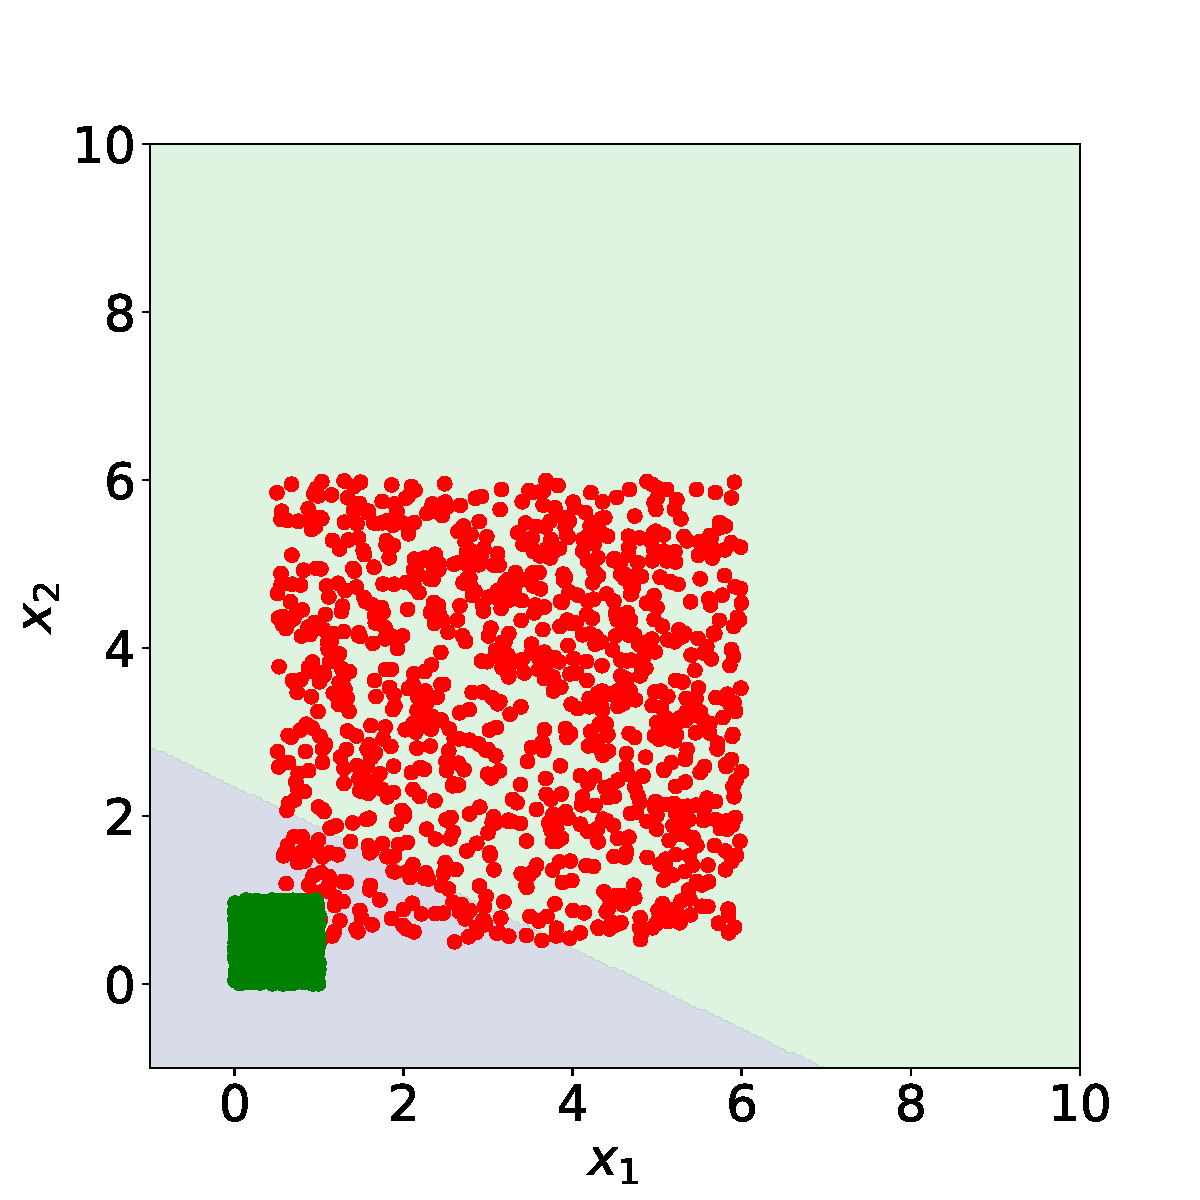
\includegraphics[width=1.5in]{../results/ex1/samples_LOG_dataset_Uniform_size_10.pdf}
       \caption{LOG Classifier}
       \label{fig:LOGD_P1a_10}
    \end{subfigure}
    
    \begin{subfigure}[!htbp]{0.2\textwidth}
       \centering
       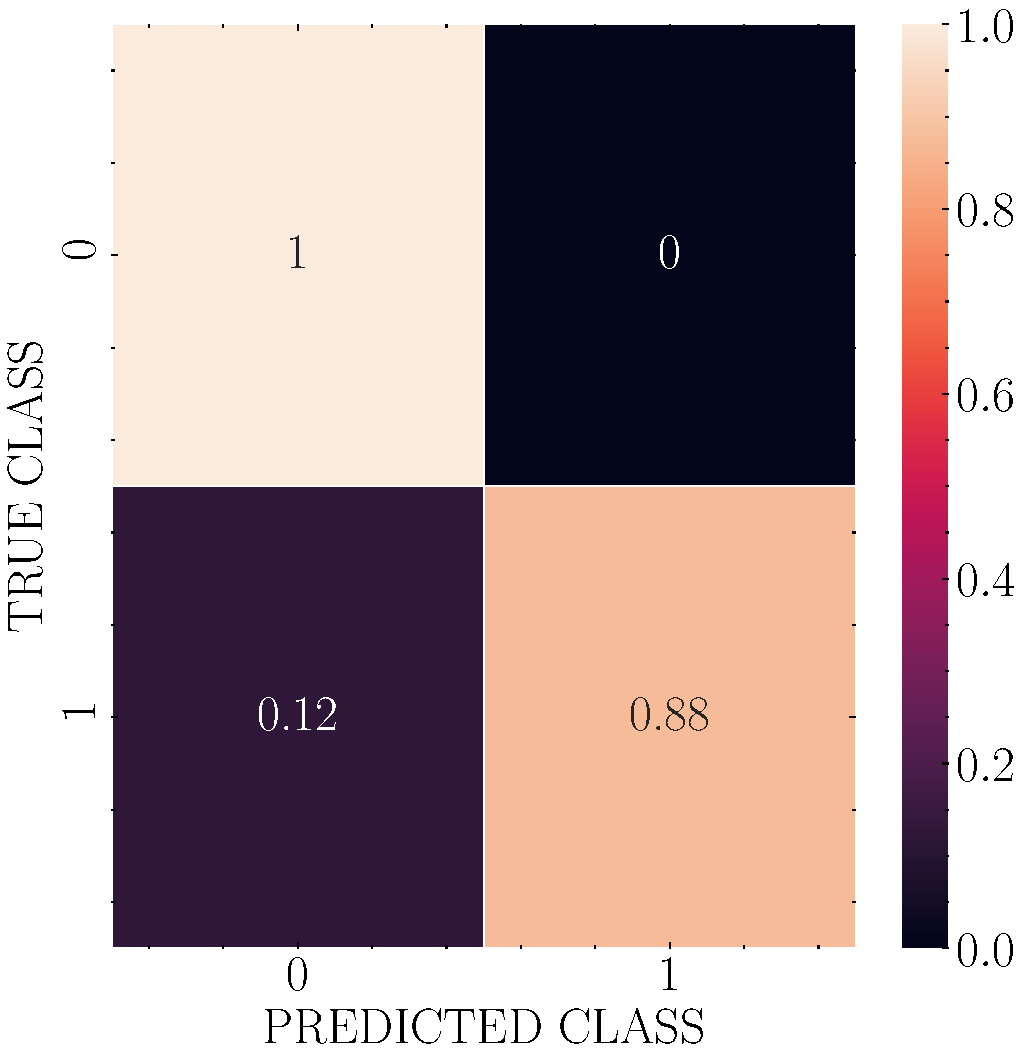
\includegraphics[width=1.5in]{../results/ex1/acc_LS_dataset_Uniform_size_50.pdf}
       \caption{LS, size $50$}
       \label{fig:LS_P1a_50}
    \end{subfigure}
\quad
    \begin{subfigure}[!htbp]{0.2\textwidth}
       \centering
       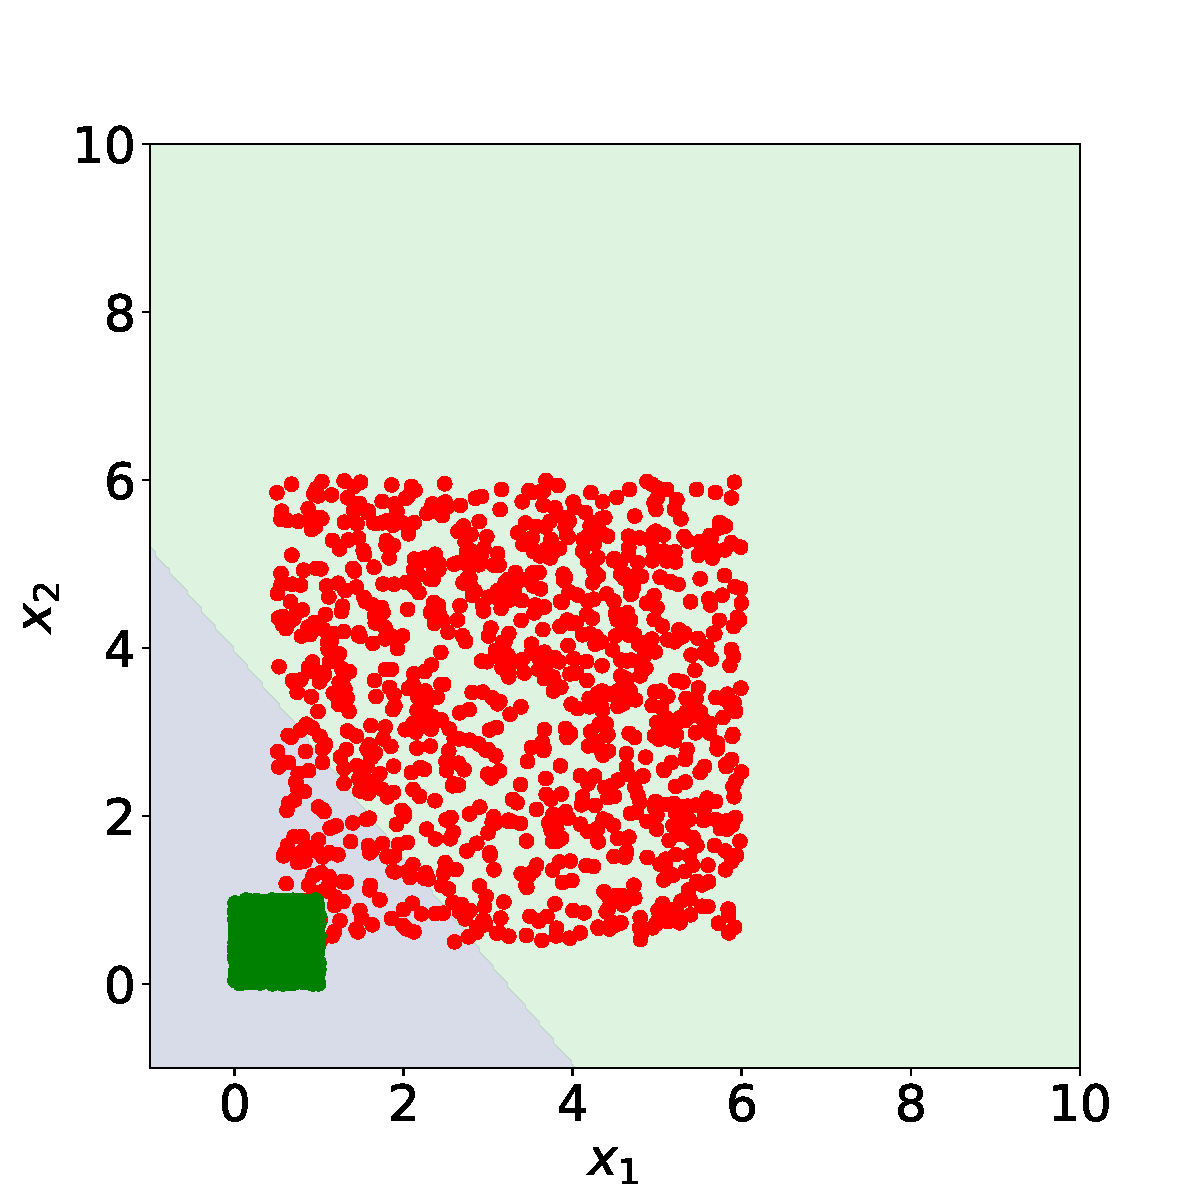
\includegraphics[width=1.5in]{../results/ex1/samples_LS_dataset_Uniform_size_50.pdf}
       \caption{LS Classifier}
       \label{fig:LSD_P1a_50}
    \end{subfigure}
\quad
    \begin{subfigure}[!htbp]{0.2\textwidth}
       \centering
       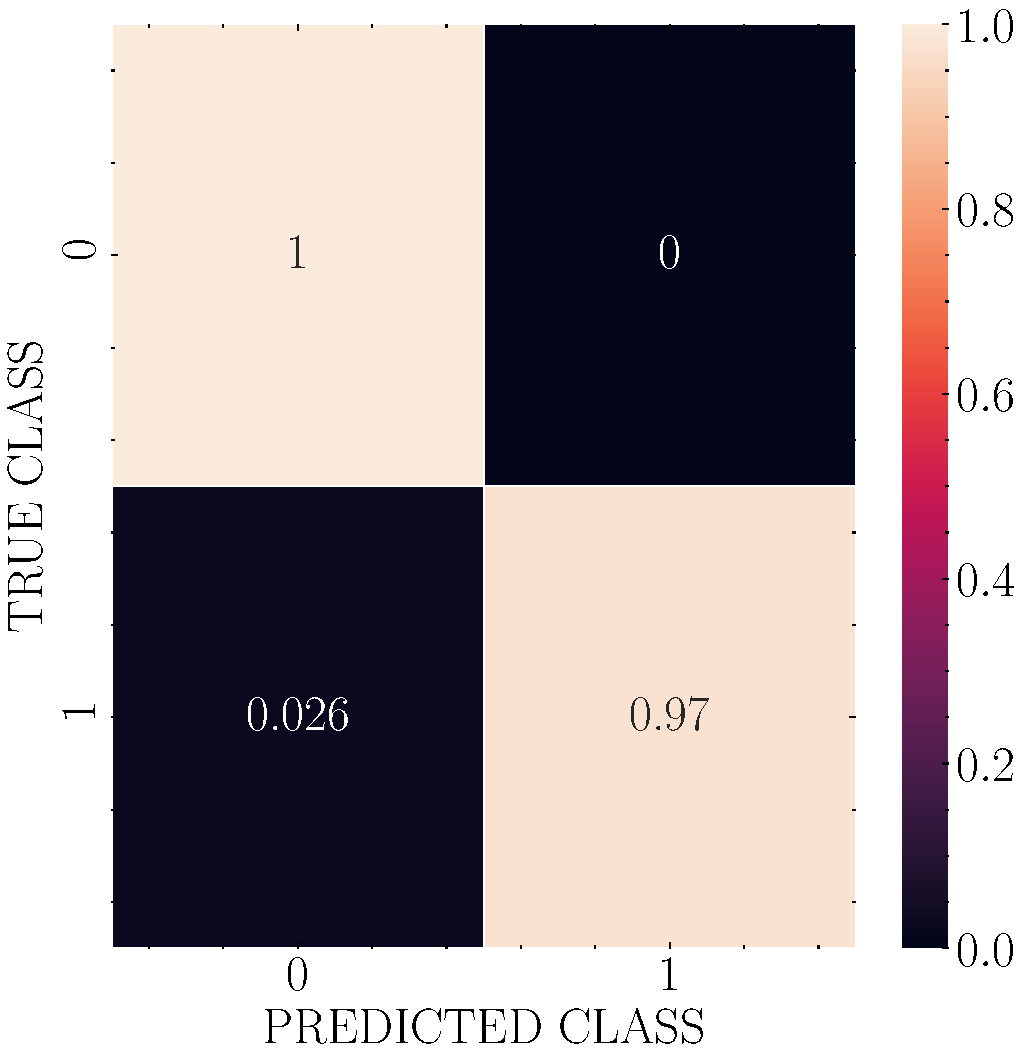
\includegraphics[width=1.5in]{../results/ex1/acc_LOG_dataset_Uniform_size_50.pdf}
       \caption{LOG, size $50$}
       \label{fig:LOG_P1a_50}
    \end{subfigure}
\quad
    \begin{subfigure}[!htbp]{0.2\textwidth}
       \centering
       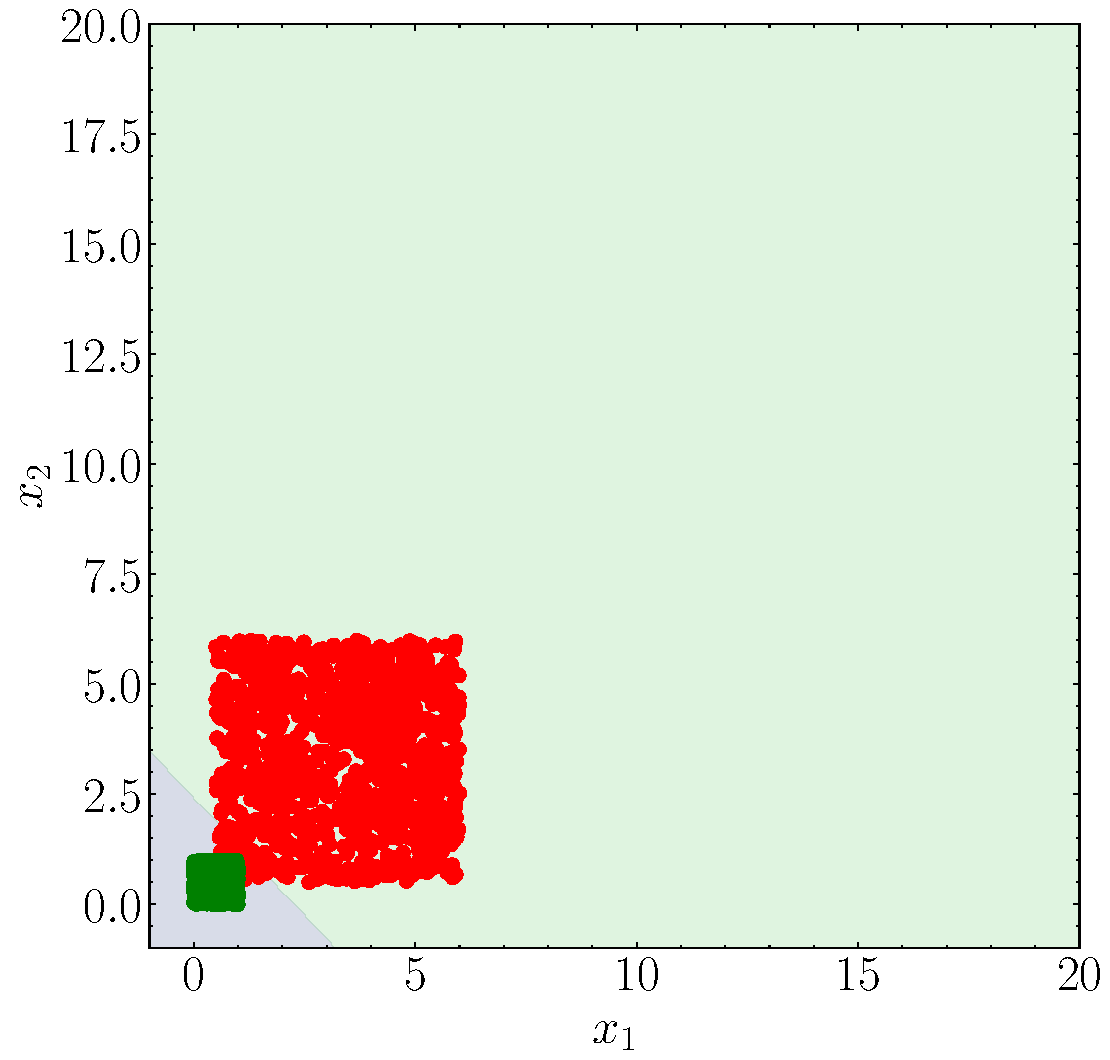
\includegraphics[width=1.5in]{../results/ex1/samples_LOG_dataset_Uniform_size_50.pdf}
       \caption{LOG Classifier}
       \label{fig:LOGD_P1a_50}
    \end{subfigure}
    
    \begin{subfigure}[!htbp]{0.2\textwidth}
       \centering
       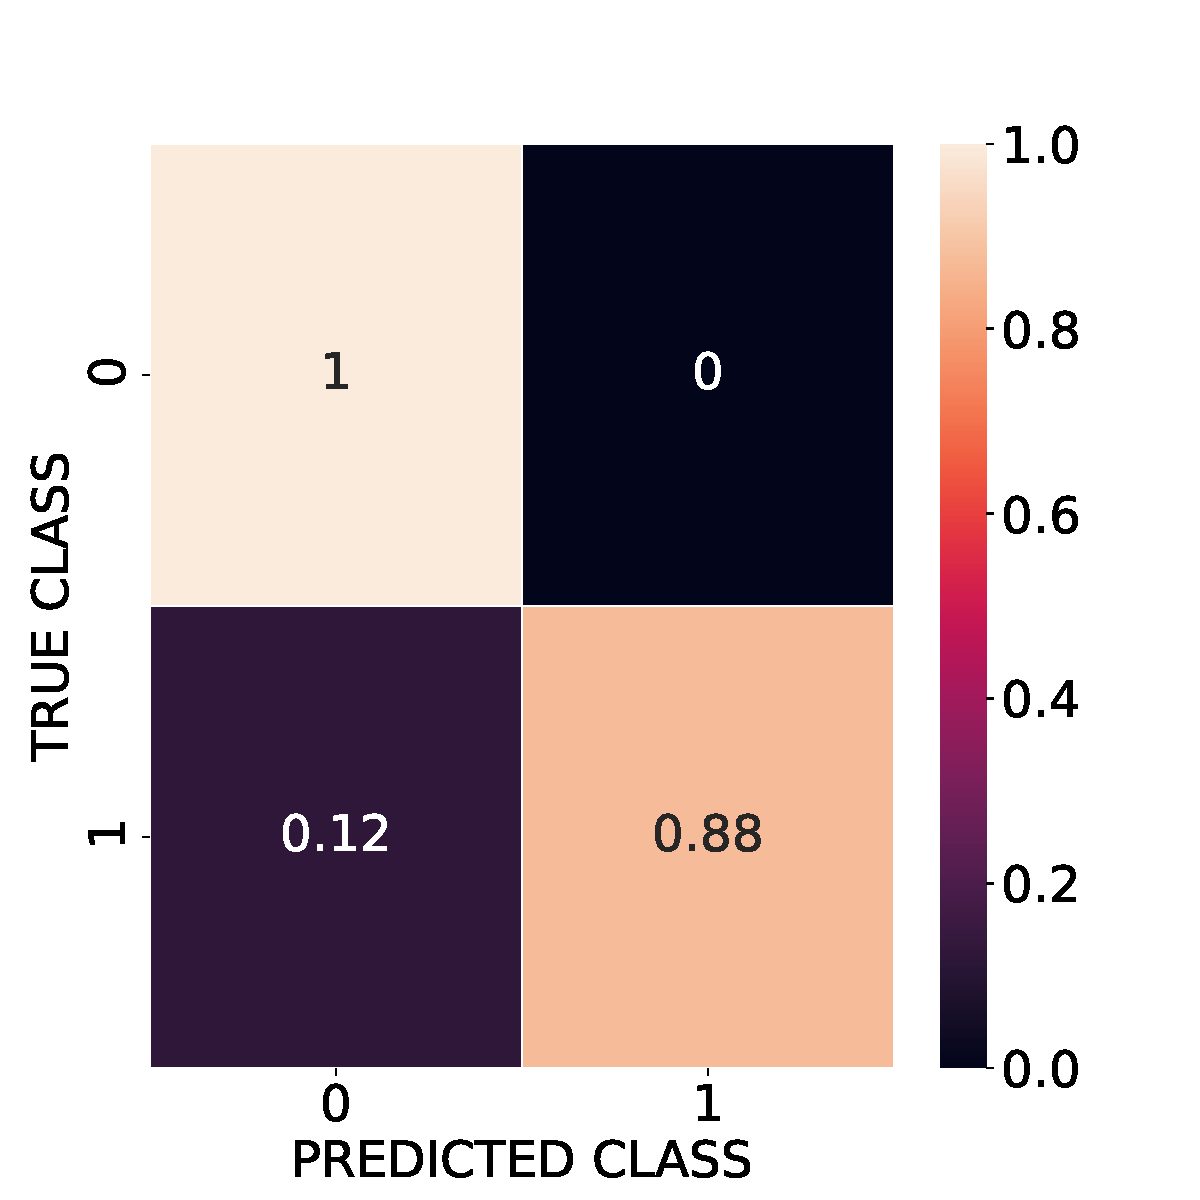
\includegraphics[width=1.5in]{../results/ex1/acc_LS_dataset_Uniform_size_100.pdf}
       \caption{LS, size $100$}
       \label{fig:LS_P1a_100}
    \end{subfigure}
\quad
    \begin{subfigure}[!htbp]{0.2\textwidth}
       \centering
       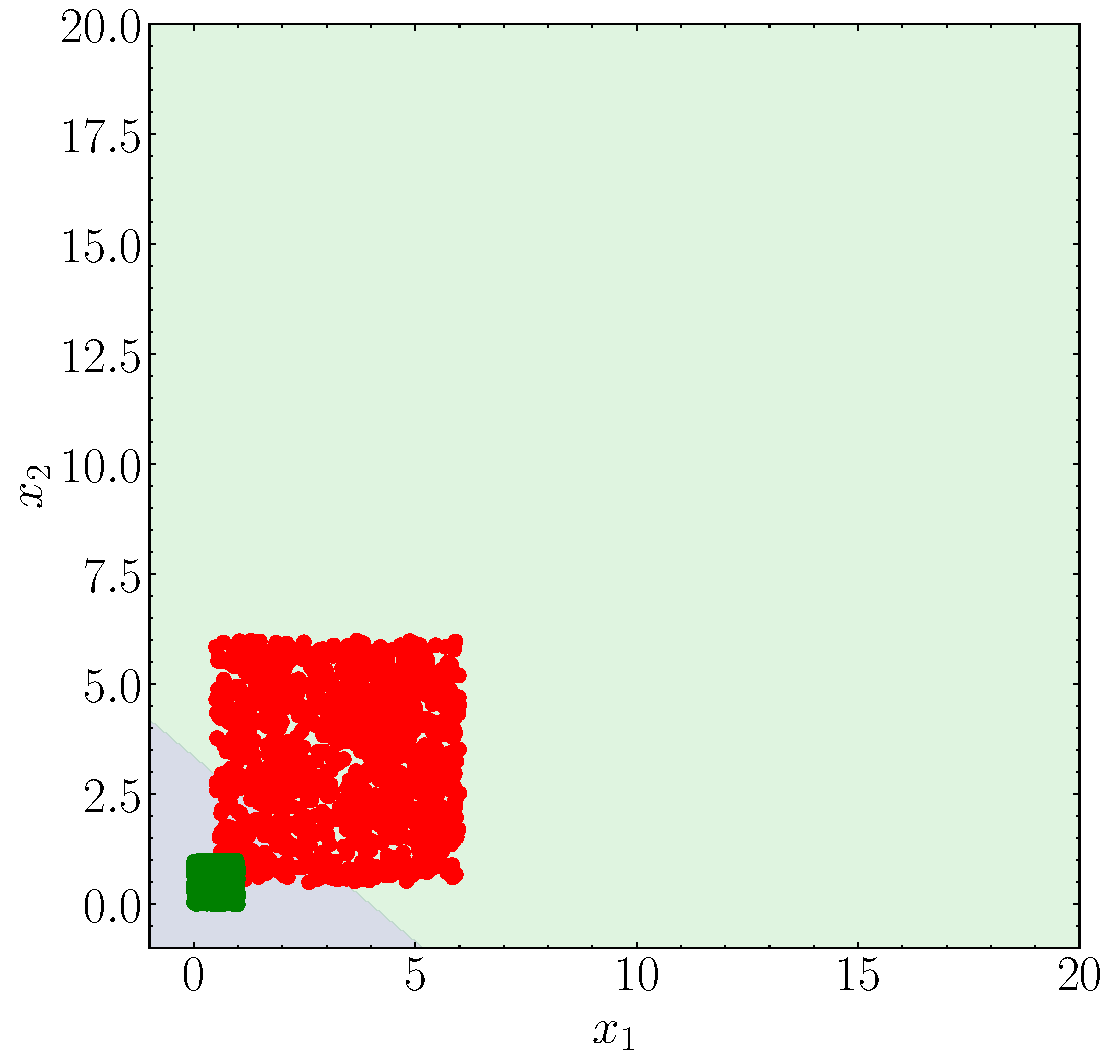
\includegraphics[width=1.5in]{../results/ex1/samples_LS_dataset_Uniform_size_100.pdf}
       \caption{LS Classifier}
       \label{fig:LSD_P1a_100}
    \end{subfigure}
\quad
    \begin{subfigure}[!htbp]{0.2\textwidth}
       \centering
       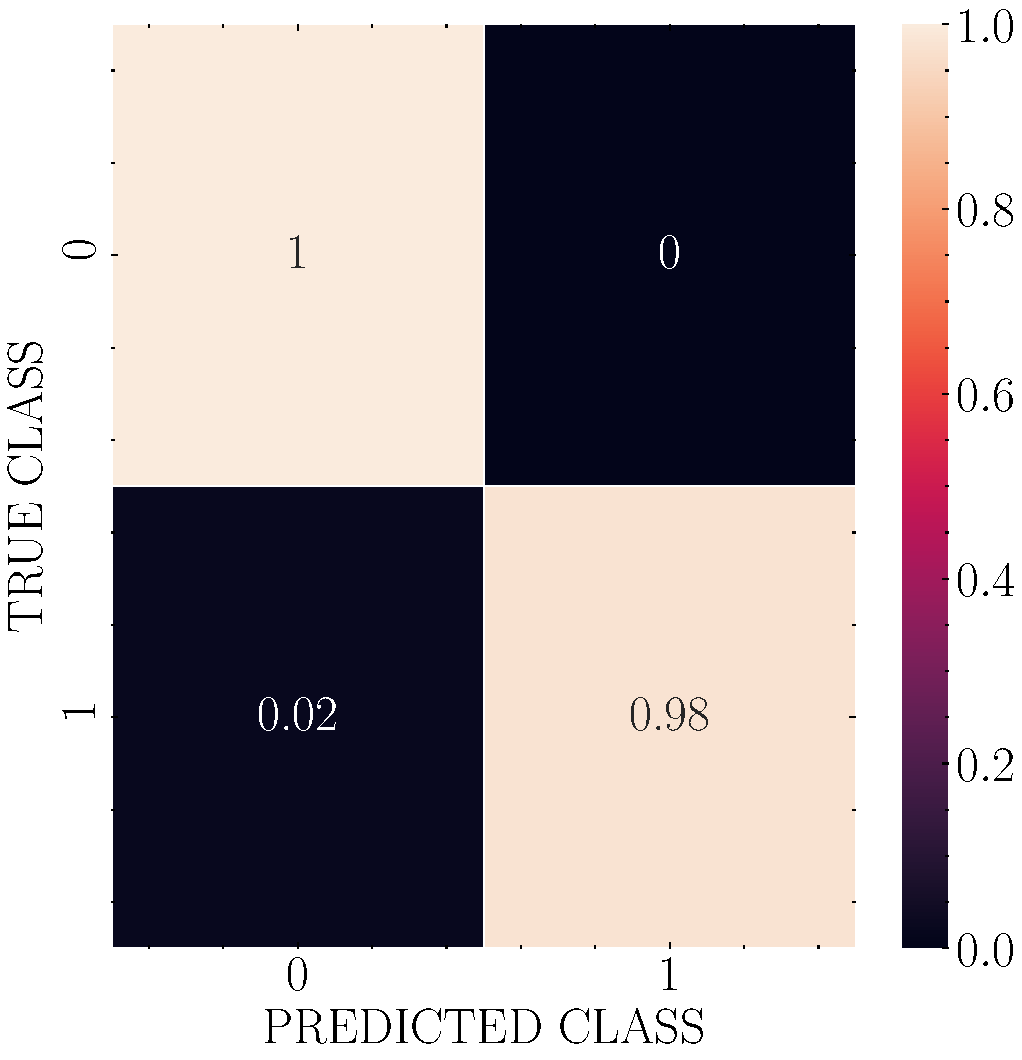
\includegraphics[width=1.5in]{../results/ex1/acc_LOG_dataset_Uniform_size_100.pdf}
       \caption{LOG, size $100$}
       \label{fig:LOG_P1a_100}
    \end{subfigure}
\quad
    \begin{subfigure}[!htbp]{0.2\textwidth}
       \centering
       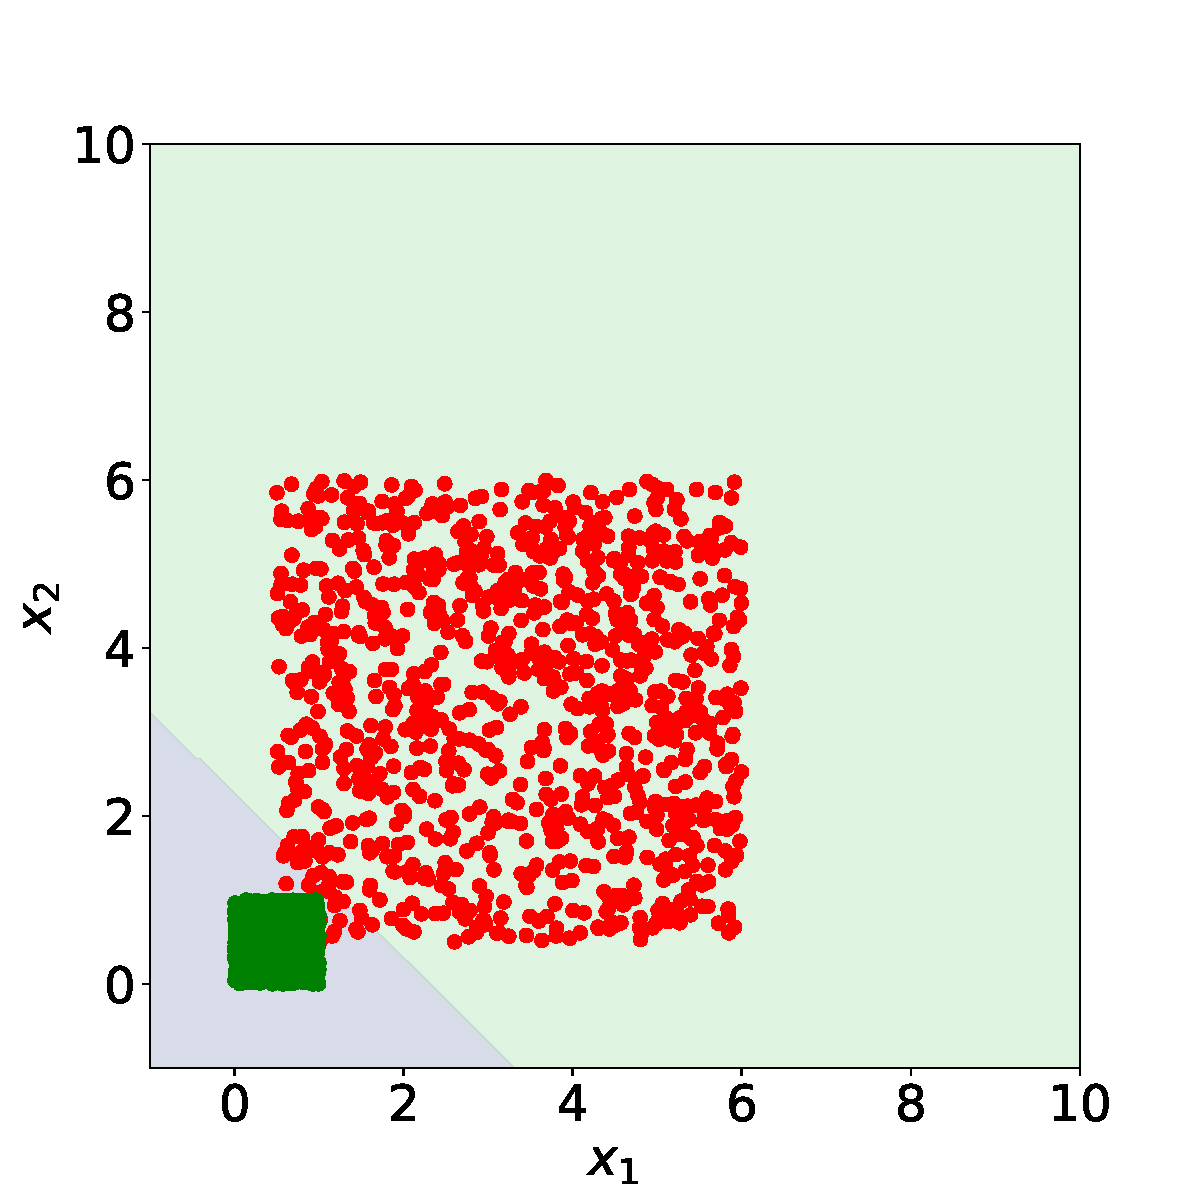
\includegraphics[width=1.5in]{../results/ex1/samples_LOG_dataset_Uniform_size_100.pdf}
       \caption{LOG Classifier}
       \label{fig:LOGD_P1a_100}
    \end{subfigure} 
    
    \begin{subfigure}[!htbp]{0.2\textwidth}
       \centering
       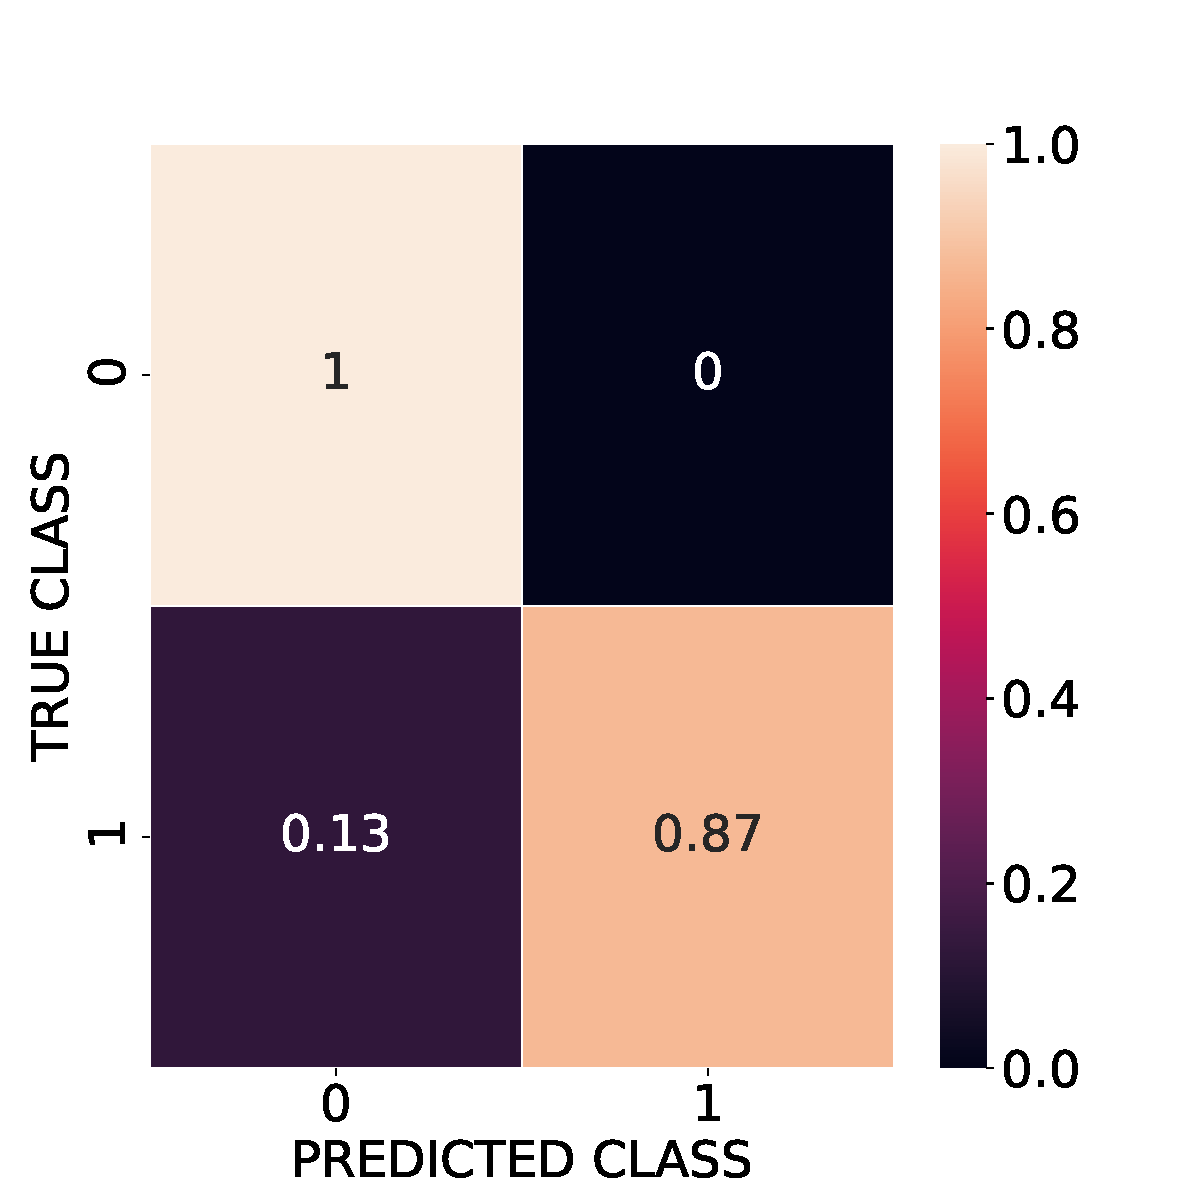
\includegraphics[width=1.5in]{../results/ex1/acc_LS_dataset_Uniform_size_500.pdf}
       \caption{LS, size $500$}
       \label{fig:LS_P1a_500}
    \end{subfigure}
\quad
    \begin{subfigure}[!htbp]{0.2\textwidth}
       \centering
       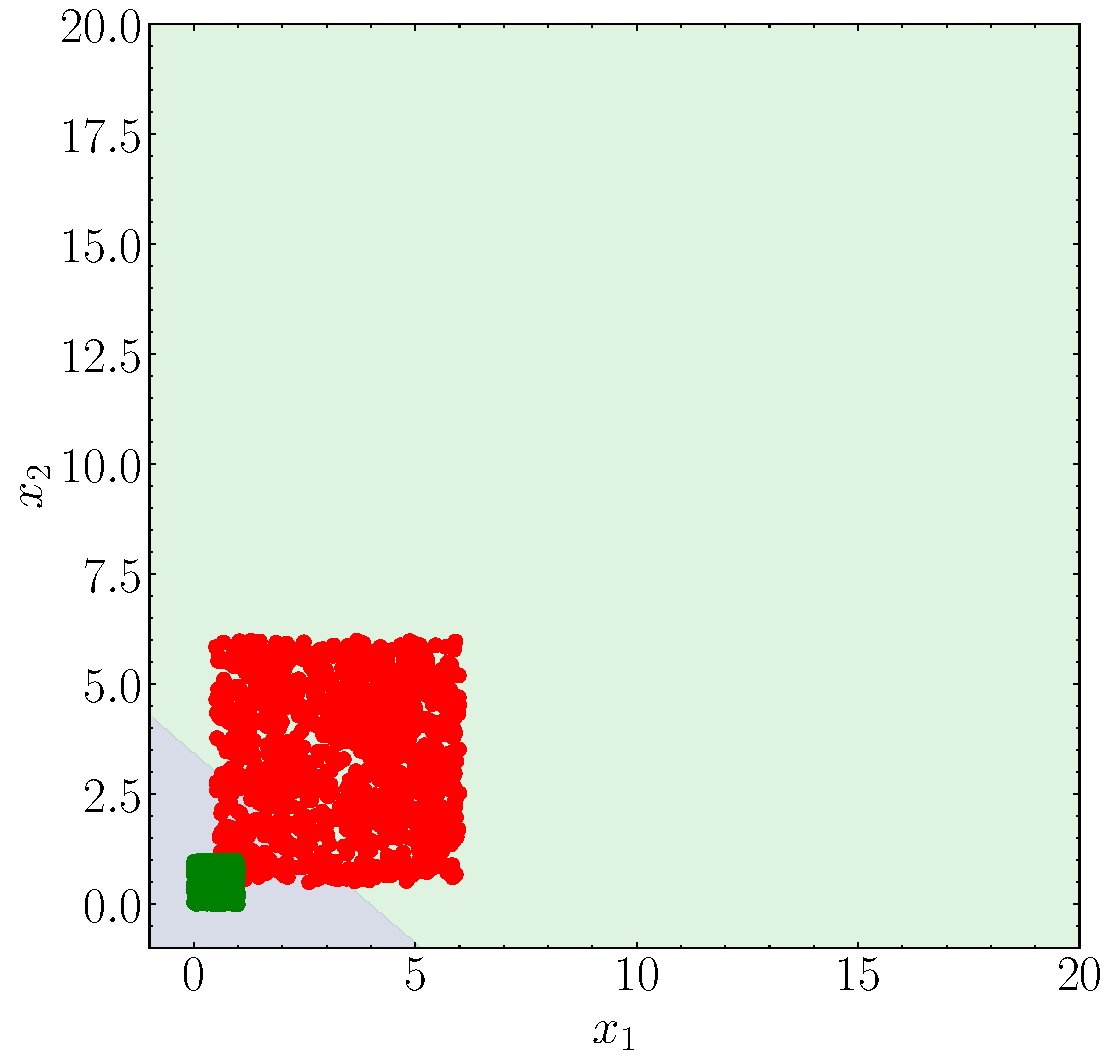
\includegraphics[width=1.5in]{../results/ex1/samples_LS_dataset_Uniform_size_500.pdf}
       \caption{LS Classifier}
       \label{fig:LSD_P1a_500}
    \end{subfigure}
\quad
    \begin{subfigure}[!htbp]{0.2\textwidth}
       \centering
       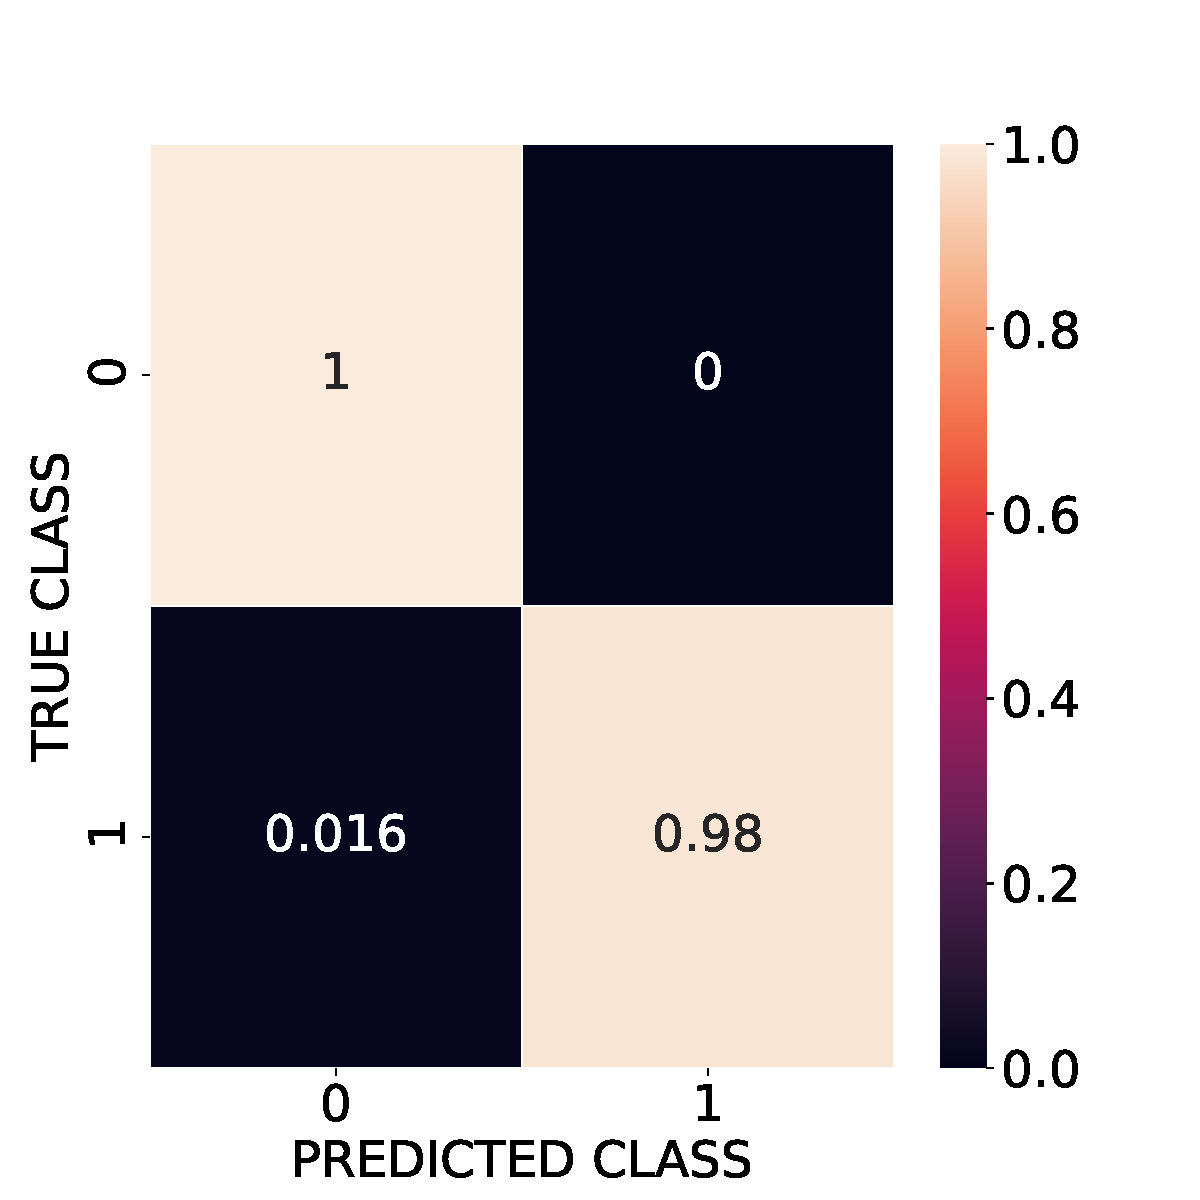
\includegraphics[width=1.5in]{../results/ex1/acc_LOG_dataset_Uniform_size_500.pdf}
       \caption{LOG, size $500$}
       \label{fig:LOG_P1a_500}
    \end{subfigure}
\quad
    \begin{subfigure}[!htbp]{0.2\textwidth}
       \centering
       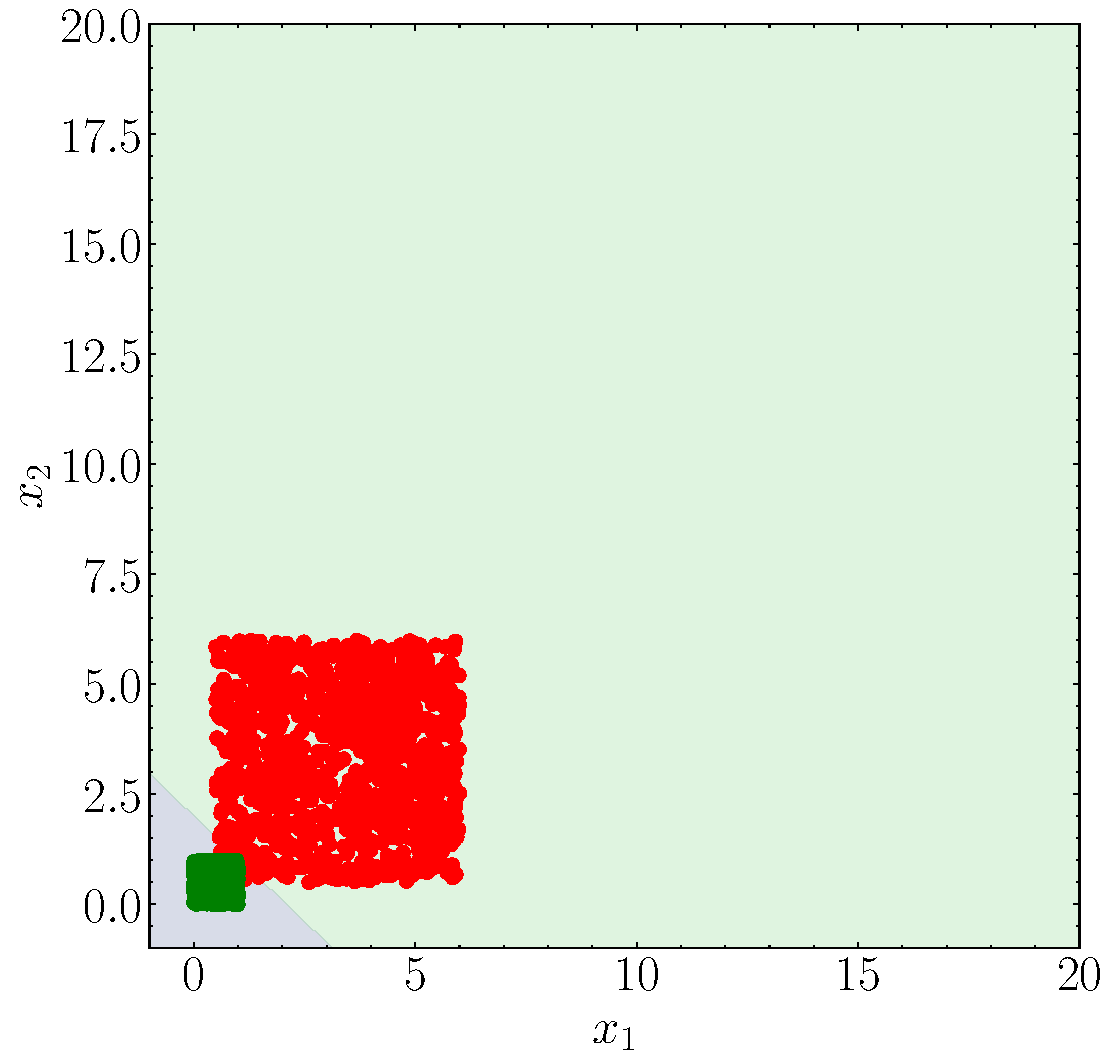
\includegraphics[width=1.5in]{../results/ex1/samples_LOG_dataset_Uniform_size_500.pdf}
       \caption{LOG Classifier}
       \label{fig:LOGD_P1a_500}
    \end{subfigure} 
    
    \begin{subfigure}[!htbp]{0.2\textwidth}
       \centering
       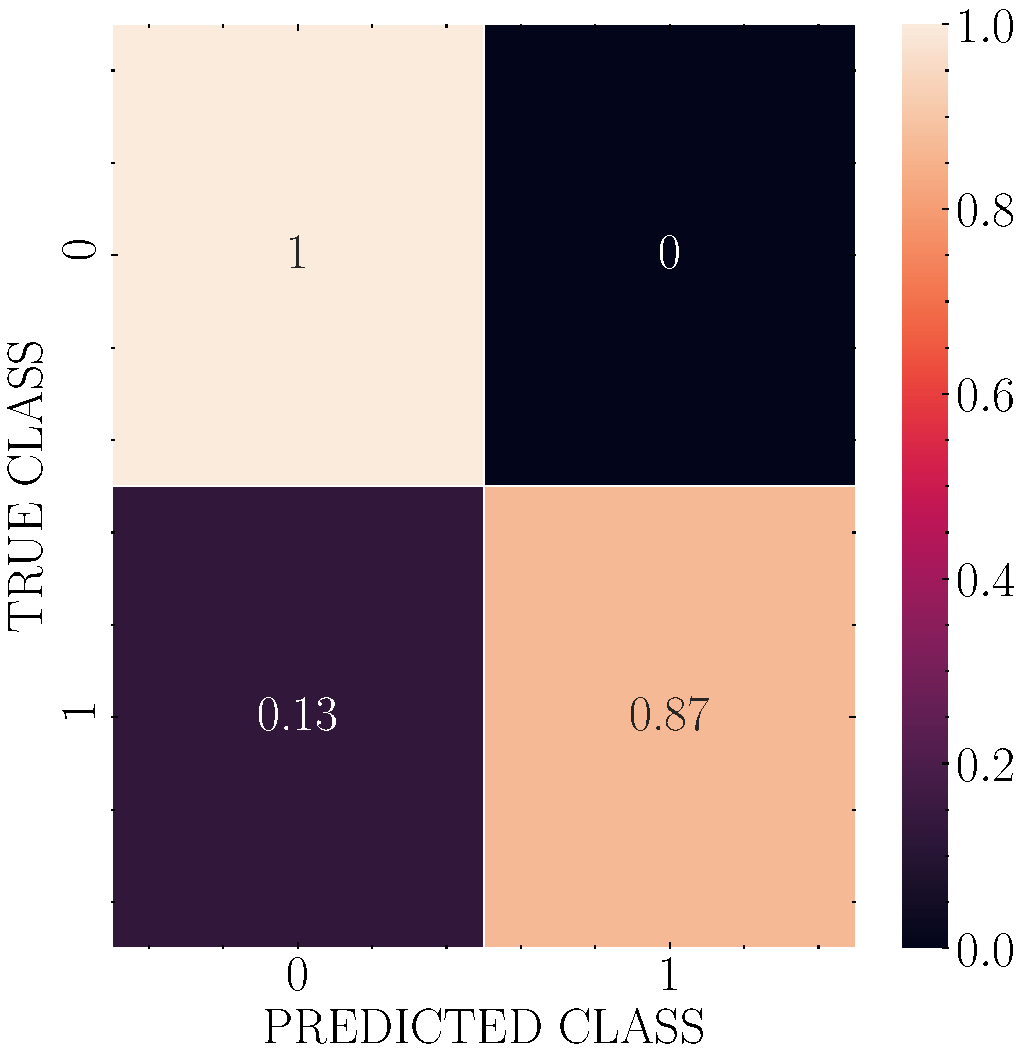
\includegraphics[width=1.5in]{../results/ex1/acc_LS_dataset_Uniform_size_999.pdf}
       \caption{LS, size $999$}
       \label{fig:LS_P1a_999}
    \end{subfigure}
\quad
    \begin{subfigure}[!htbp]{0.2\textwidth}
       \centering
       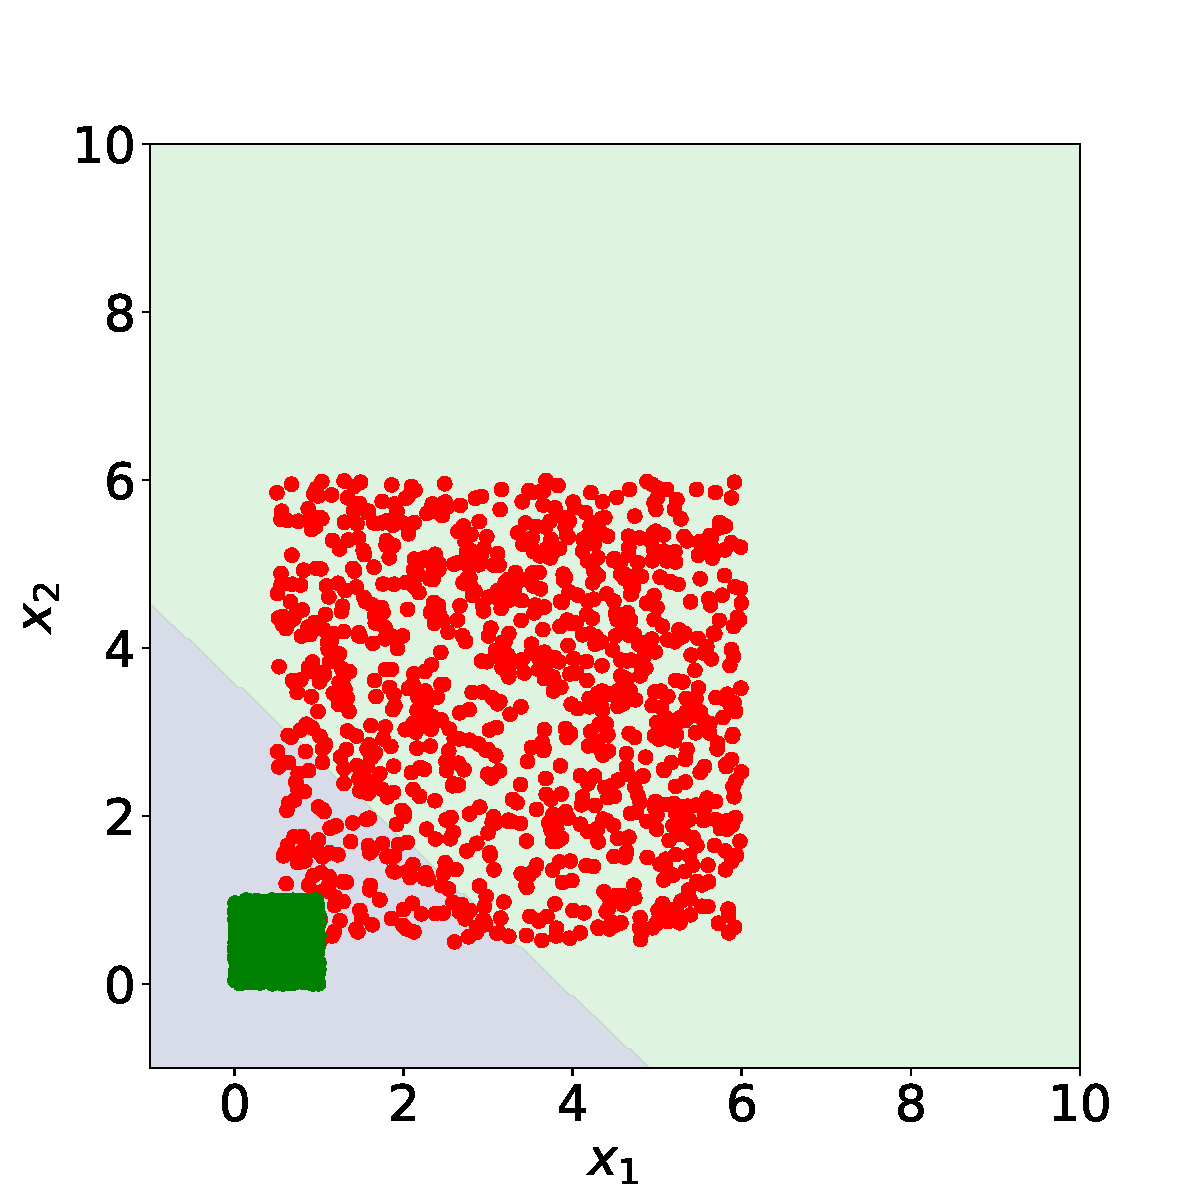
\includegraphics[width=1.5in]{../results/ex1/samples_LS_dataset_Uniform_size_999.pdf}
       \caption{LS Classifier}
       \label{fig:LSD_P1a_999}
    \end{subfigure}
\quad
    \begin{subfigure}[!htbp]{0.2\textwidth}
       \centering
       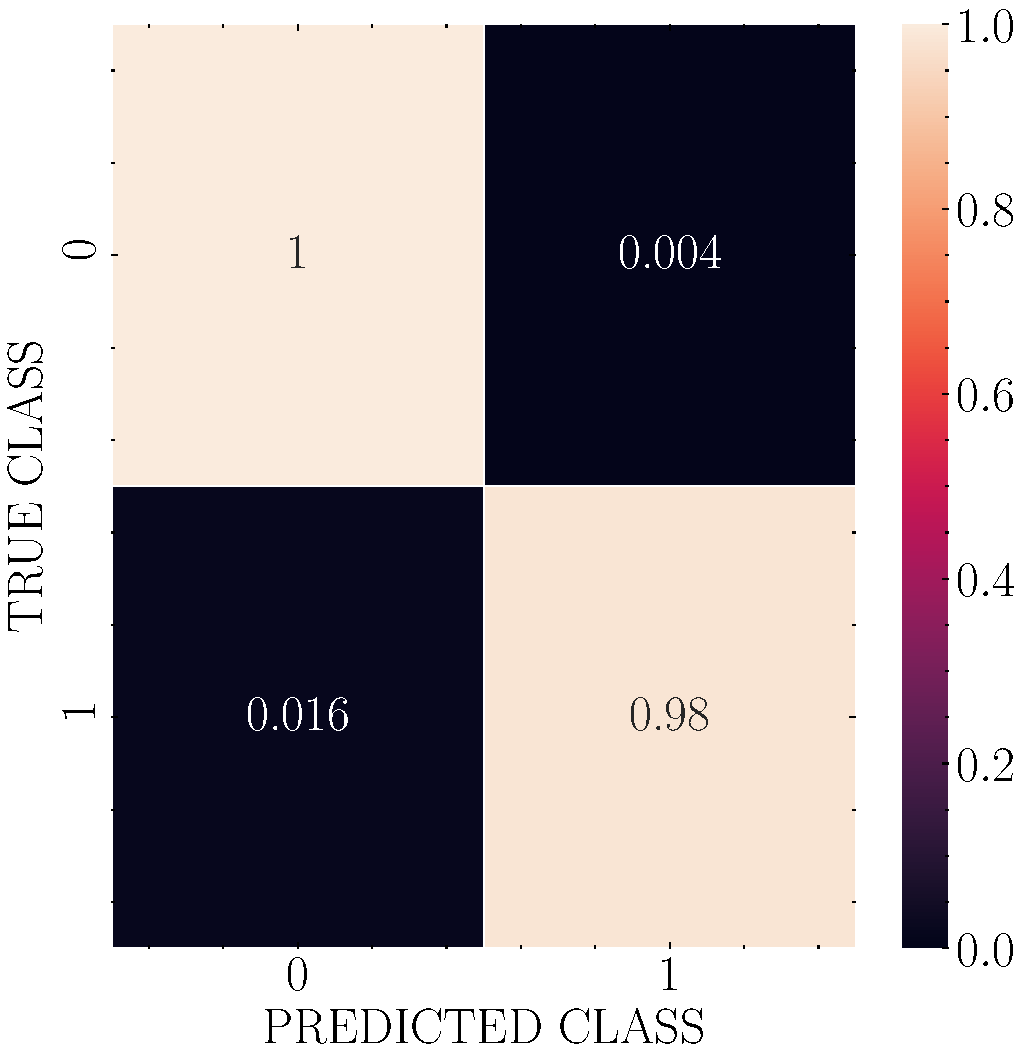
\includegraphics[width=1.5in]{../results/ex1/acc_LOG_dataset_Uniform_size_999.pdf}
       \caption{LOG, size $999$}
       \label{fig:LOG_P1a_999}
    \end{subfigure}
\quad
    \begin{subfigure}[!htbp]{0.2\textwidth}
       \centering
       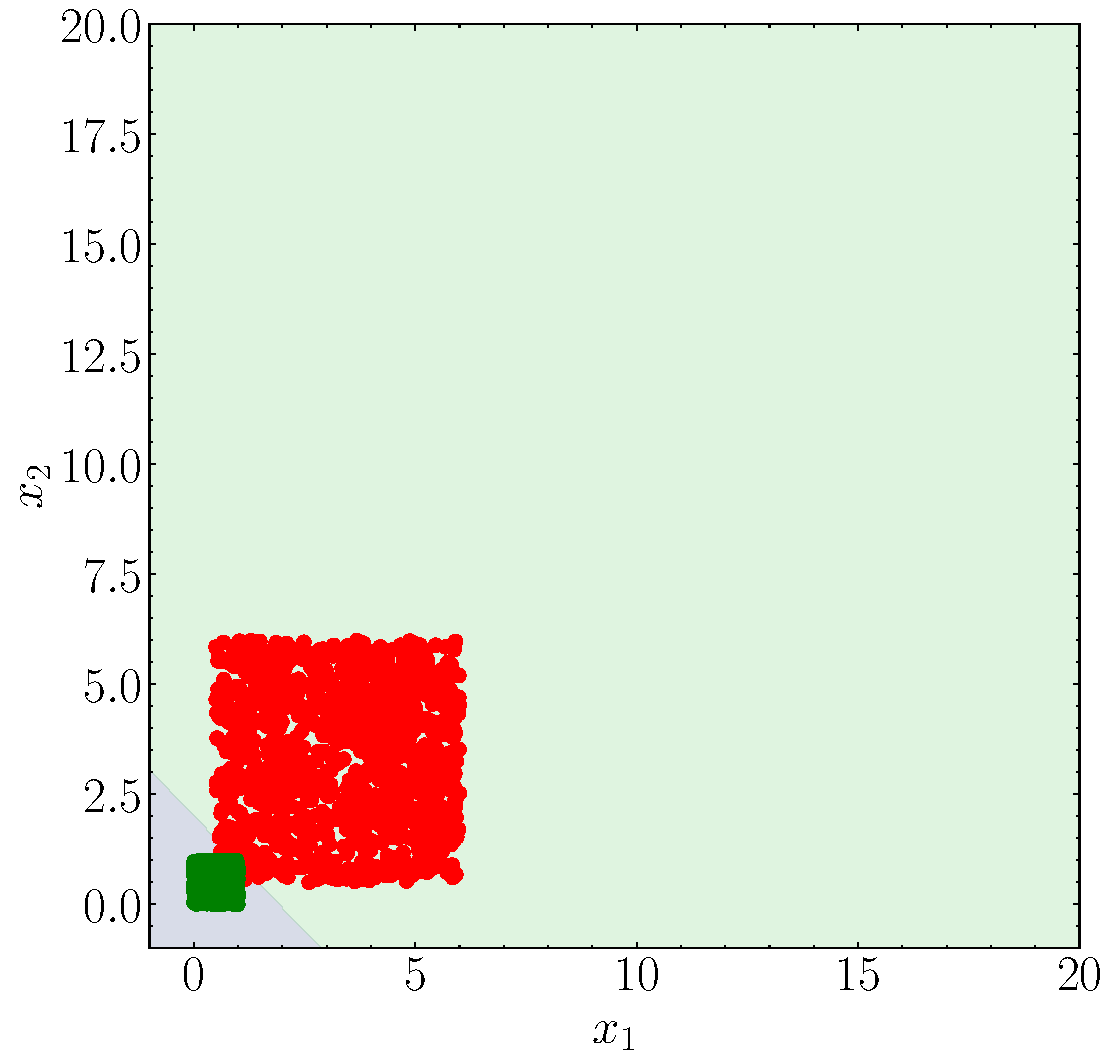
\includegraphics[width=1.5in]{../results/ex1/samples_LOG_dataset_Uniform_size_999.pdf}
       \caption{LOG Classifier}
       \label{fig:LOGD_P1a_999}
    \end{subfigure}     

\caption{Linear Least-Squares Classification and Logistic Regression.}
\label{fig:ex1_P1a}
\end{figure}

% ------------------------------------------------------------------------------------------------------------------------------------------------------

\problem{Problem (1.c) Gaussian-distributed Classes in 10D}
\label{prob:1.c}

\begin{figure}[!htbp]
\centering
    \begin{subfigure}[!htbp]{0.2\textwidth}
       \centering
       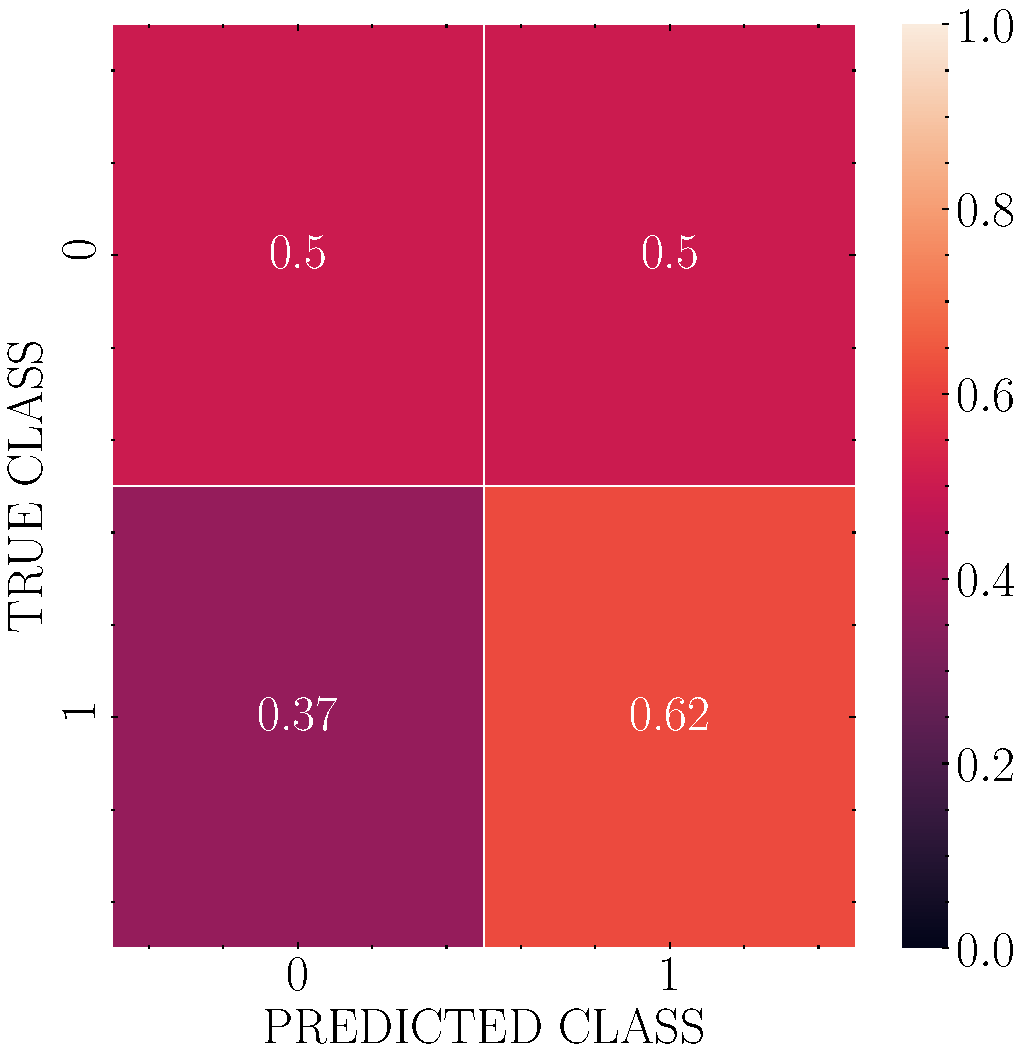
\includegraphics[width=1.5in]{../results/ex1/acc_LS_dataset_Normal_size_10.pdf}
       \caption{LS, size $10$}
       \label{fig:LS_P1a_10}
    \end{subfigure}
\quad
    \begin{subfigure}[!htbp]{0.2\textwidth}
       \centering
       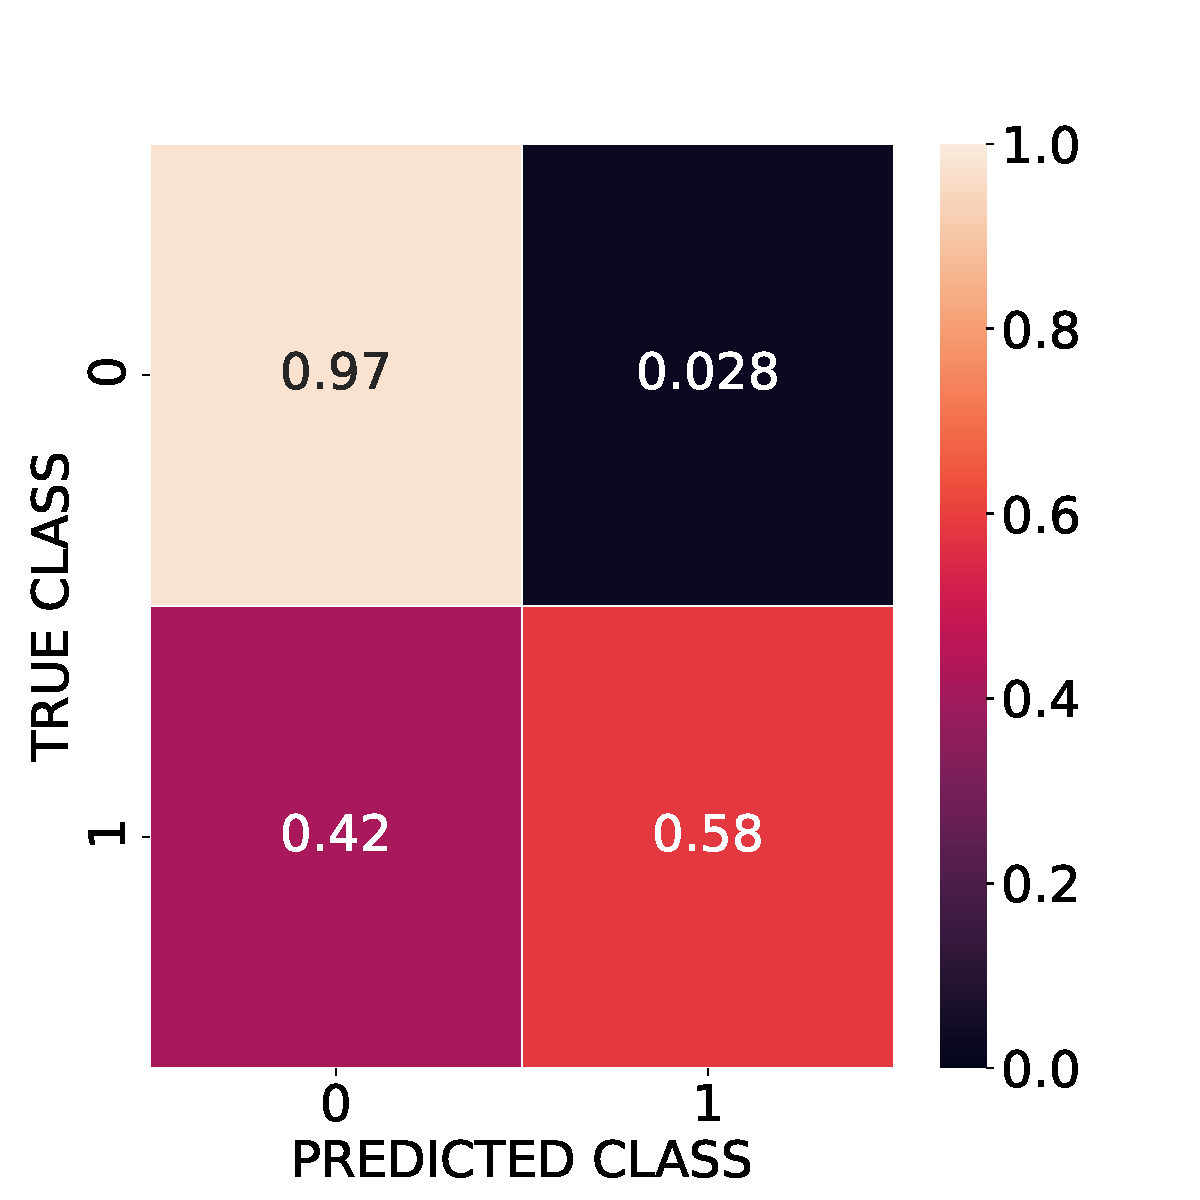
\includegraphics[width=1.5in]{../results/ex1/acc_LOG_dataset_Normal_size_10.pdf}
       \caption{LOG, size $10$}
       \label{fig:LOG_P1a_10}
    \end{subfigure}
\quad  
    \begin{subfigure}[!htbp]{0.2\textwidth}
       \centering
       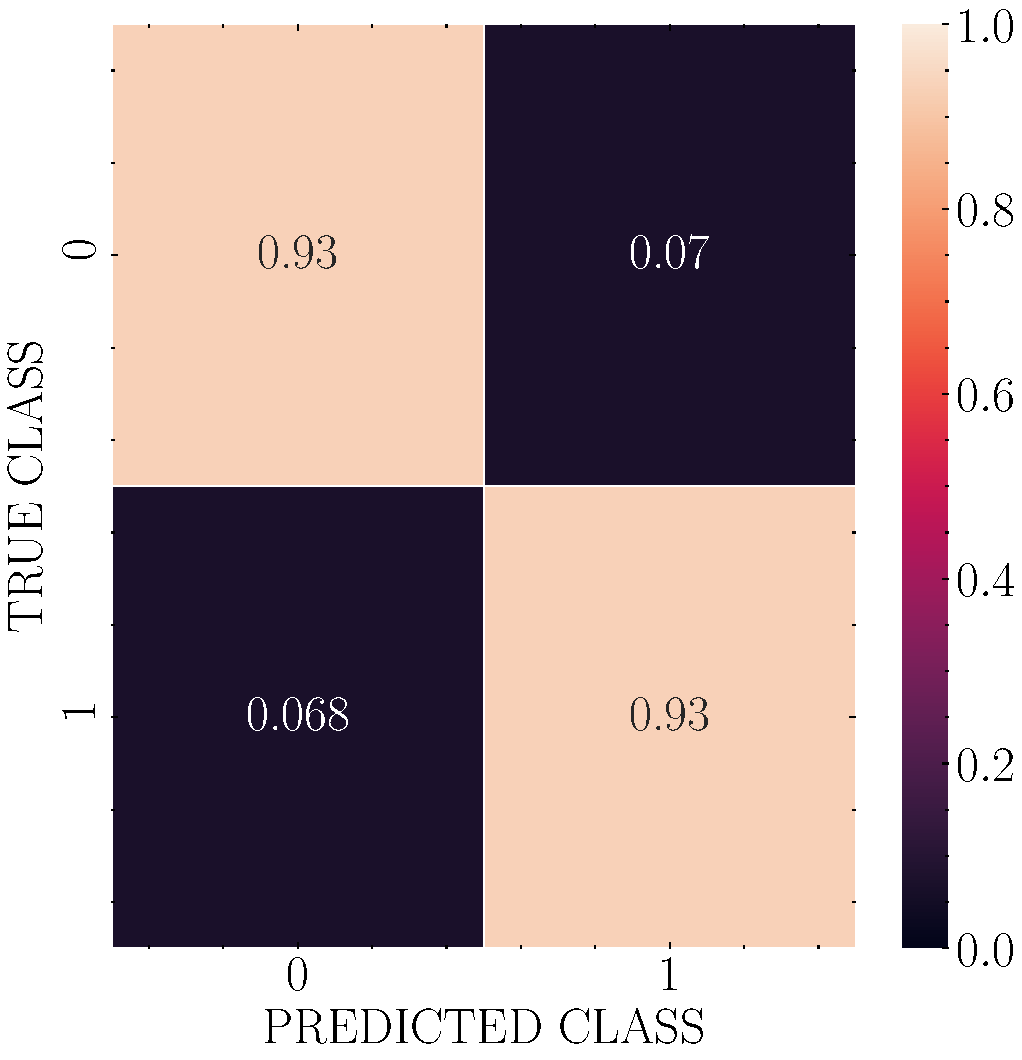
\includegraphics[width=1.5in]{../results/ex1/acc_LS_dataset_Normal_size_50.pdf}
       \caption{LS, size $50$}
       \label{fig:LS_P1a_50}
    \end{subfigure}
\quad
    \begin{subfigure}[!htbp]{0.2\textwidth}
       \centering
       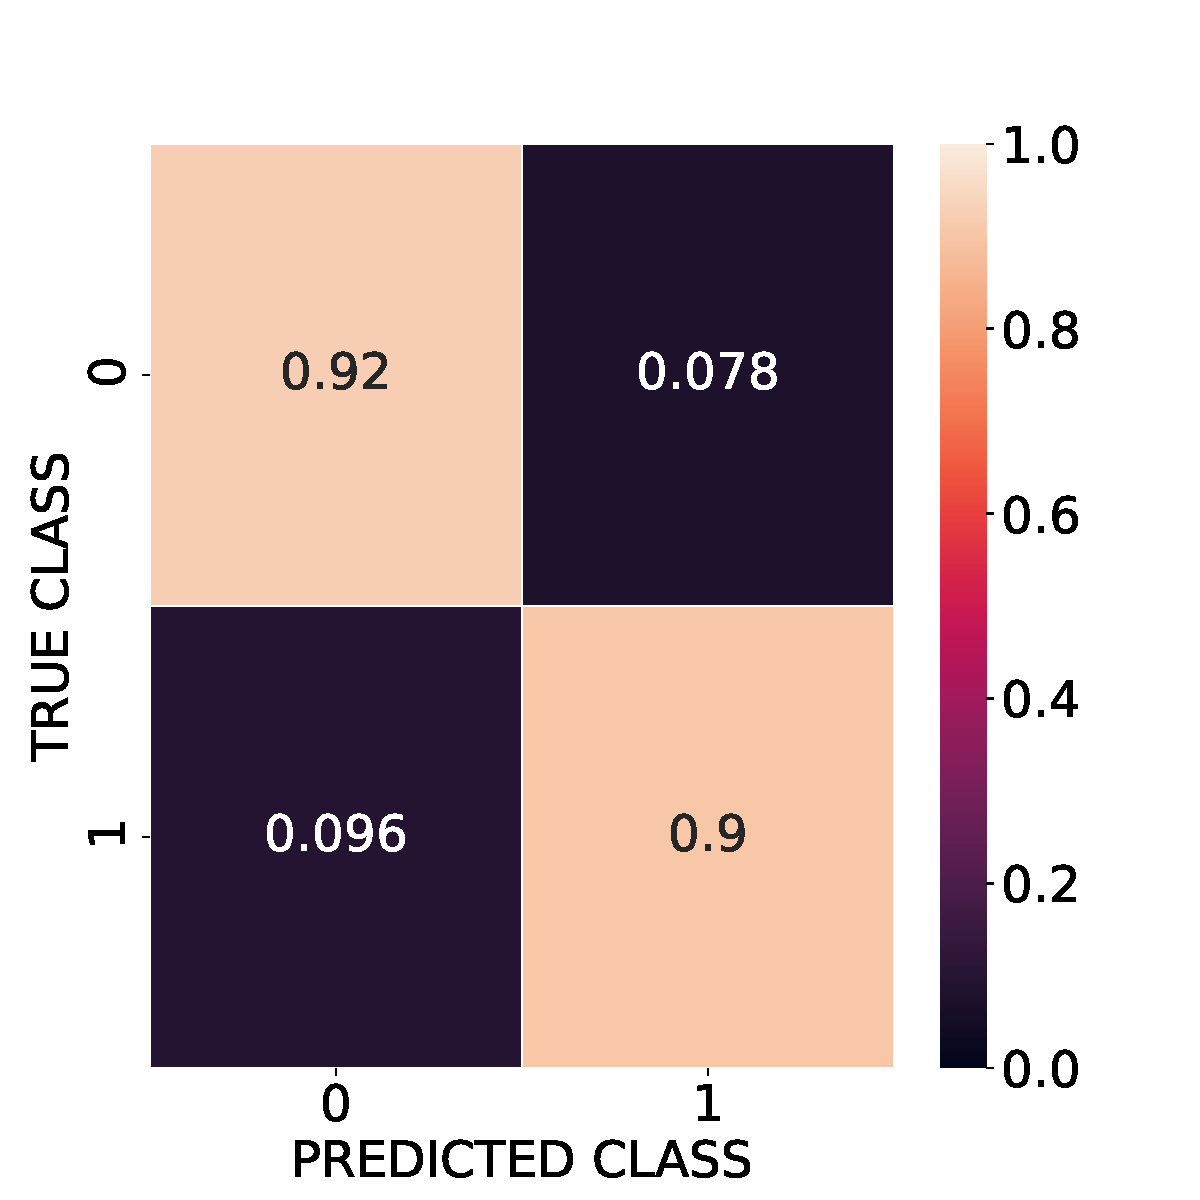
\includegraphics[width=1.5in]{../results/ex1/acc_LOG_dataset_Normal_size_50.pdf}
       \caption{LOG, size $50$}
       \label{fig:LOG_P1a_50}
    \end{subfigure}
\quad   
    \begin{subfigure}[!htbp]{0.2\textwidth}
       \centering
       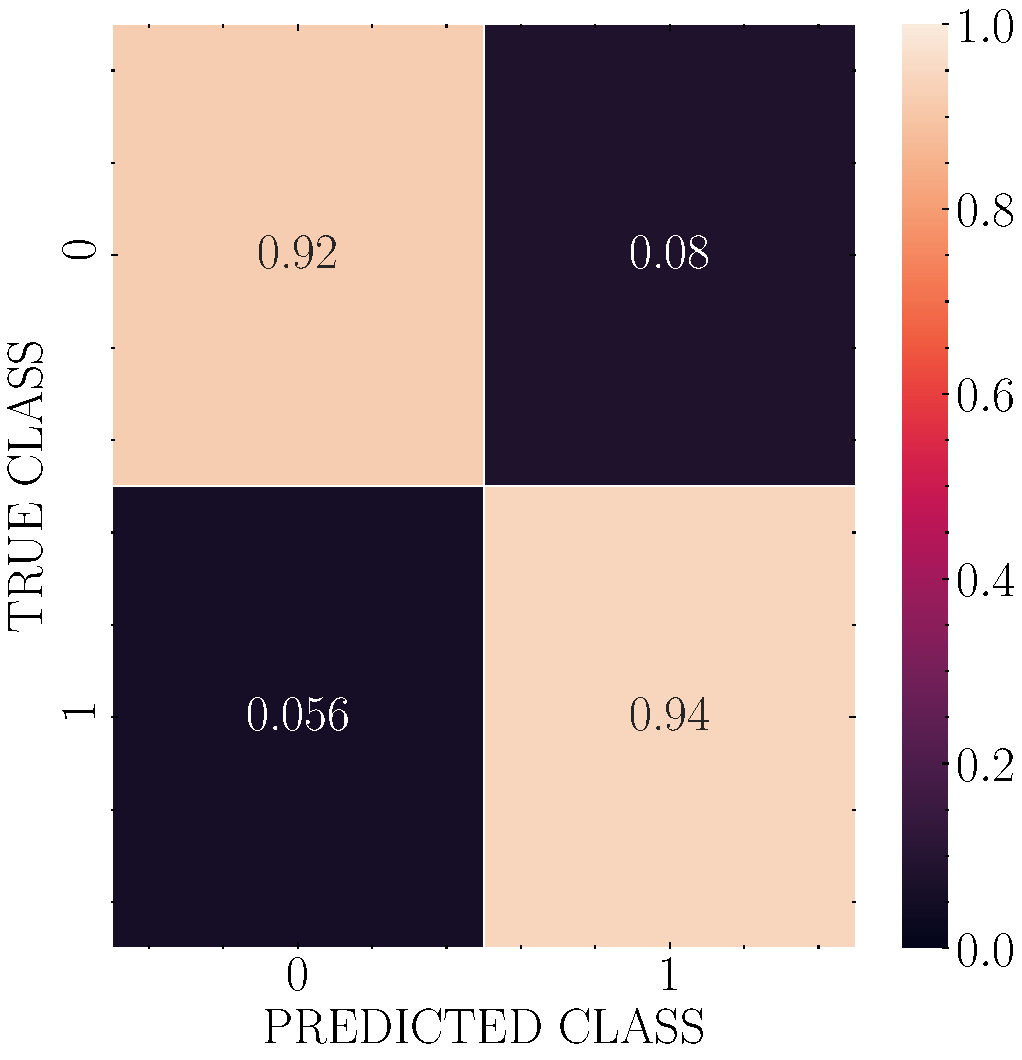
\includegraphics[width=1.5in]{../results/ex1/acc_LS_dataset_Normal_size_100.pdf}
       \caption{LS, size $100$}
       \label{fig:LS_P1a_100}
    \end{subfigure}
\quad
    \begin{subfigure}[!htbp]{0.2\textwidth}
       \centering
       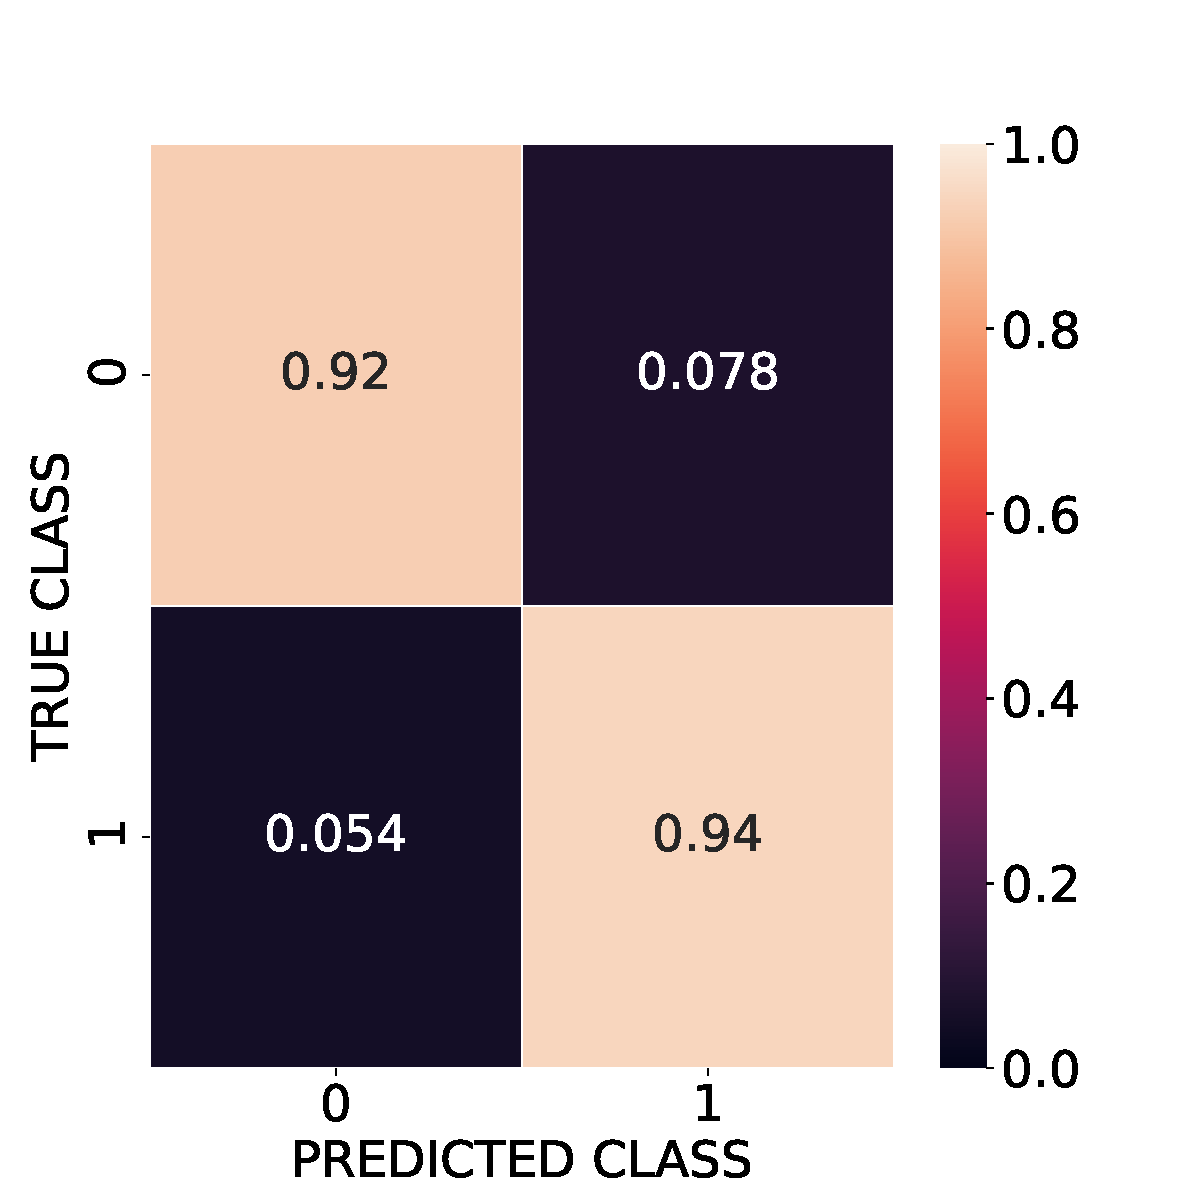
\includegraphics[width=1.5in]{../results/ex1/acc_LOG_dataset_Normal_size_100.pdf}
       \caption{LOG, size $100$}
       \label{fig:LOG_P1a_100}
    \end{subfigure}
\quad
    \begin{subfigure}[!htbp]{0.2\textwidth}
       \centering
       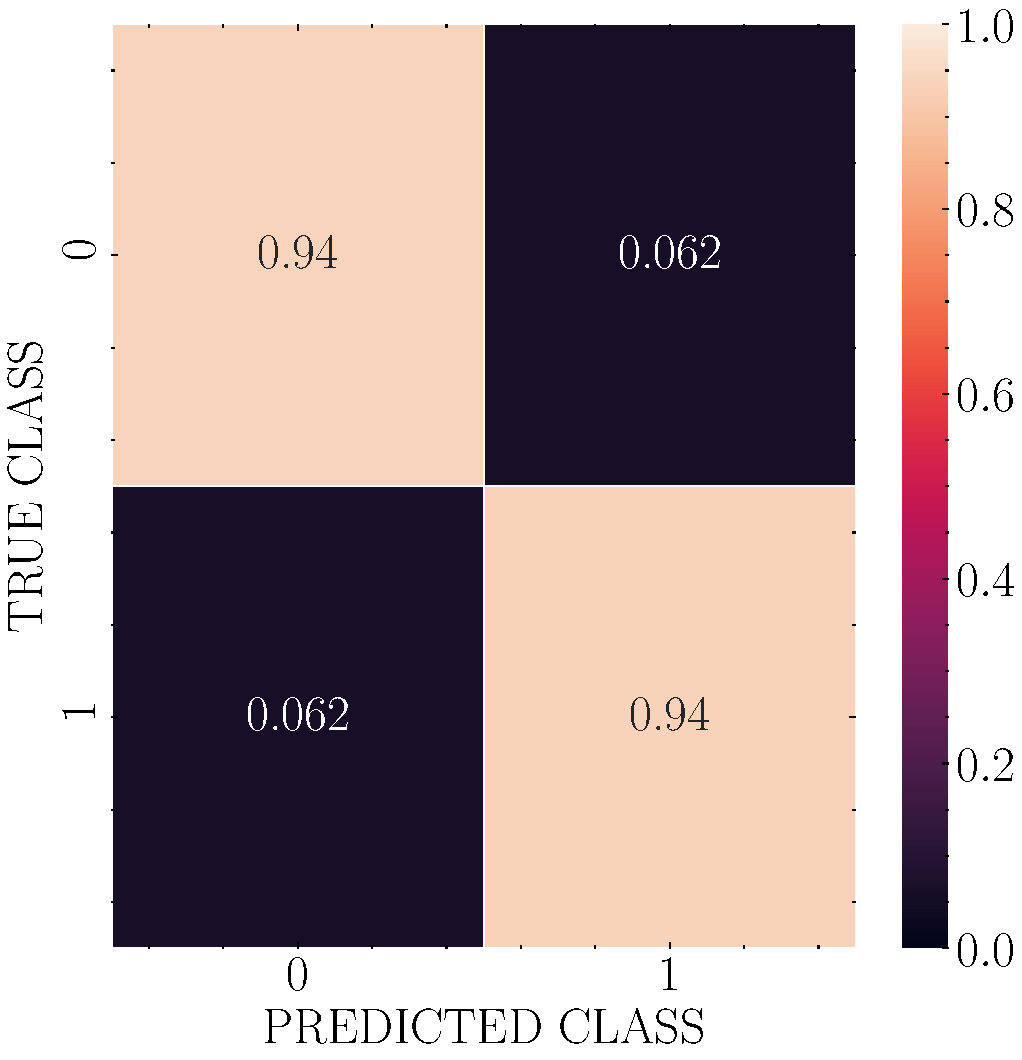
\includegraphics[width=1.5in]{../results/ex1/acc_LS_dataset_Normal_size_500.pdf}
       \caption{LS, size $500$}
       \label{fig:LS_P1a_500}
    \end{subfigure}
\quad
    \begin{subfigure}[!htbp]{0.2\textwidth}
       \centering
       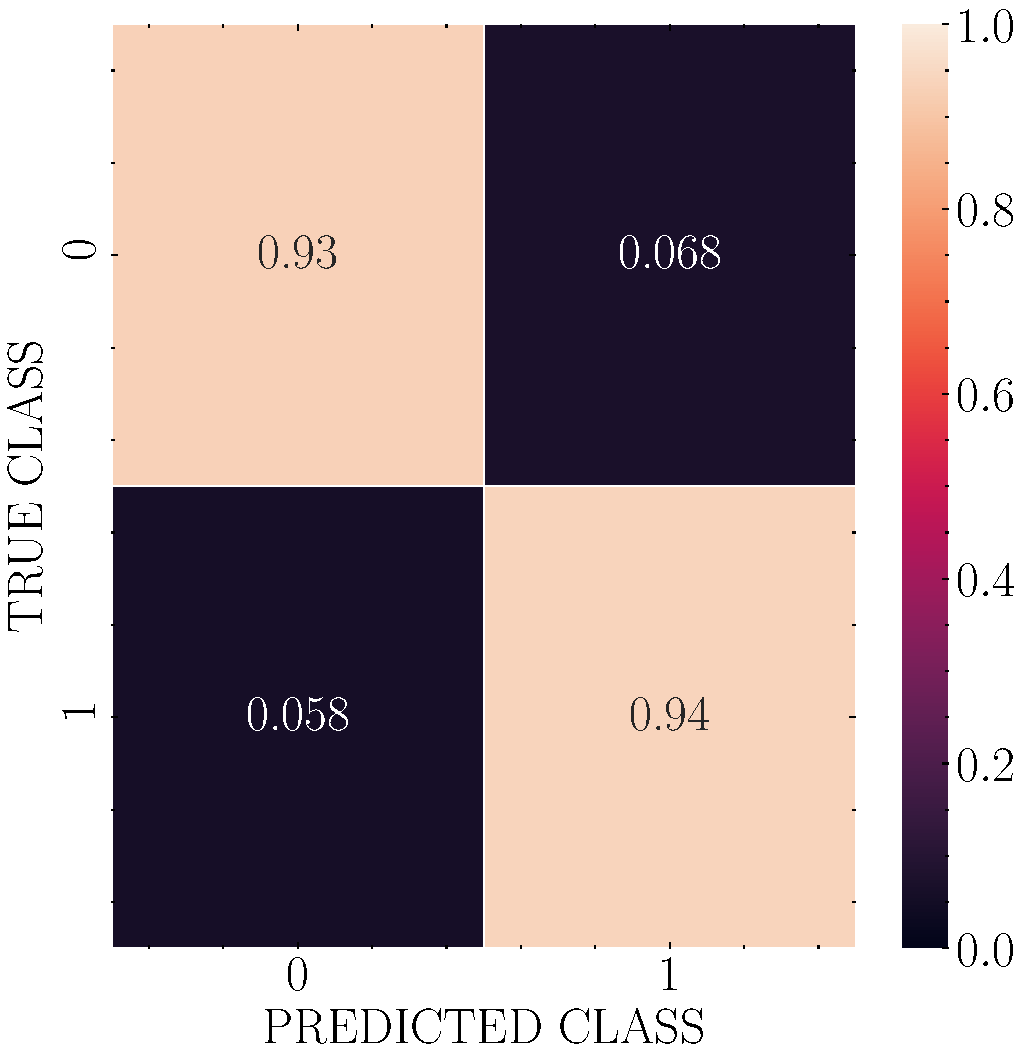
\includegraphics[width=1.5in]{../results/ex1/acc_LOG_dataset_Normal_size_500.pdf}
       \caption{LOG, size $500$}
       \label{fig:LOG_P1a_500}
    \end{subfigure}
\quad   
    \begin{subfigure}[!htbp]{0.2\textwidth}
       \centering
       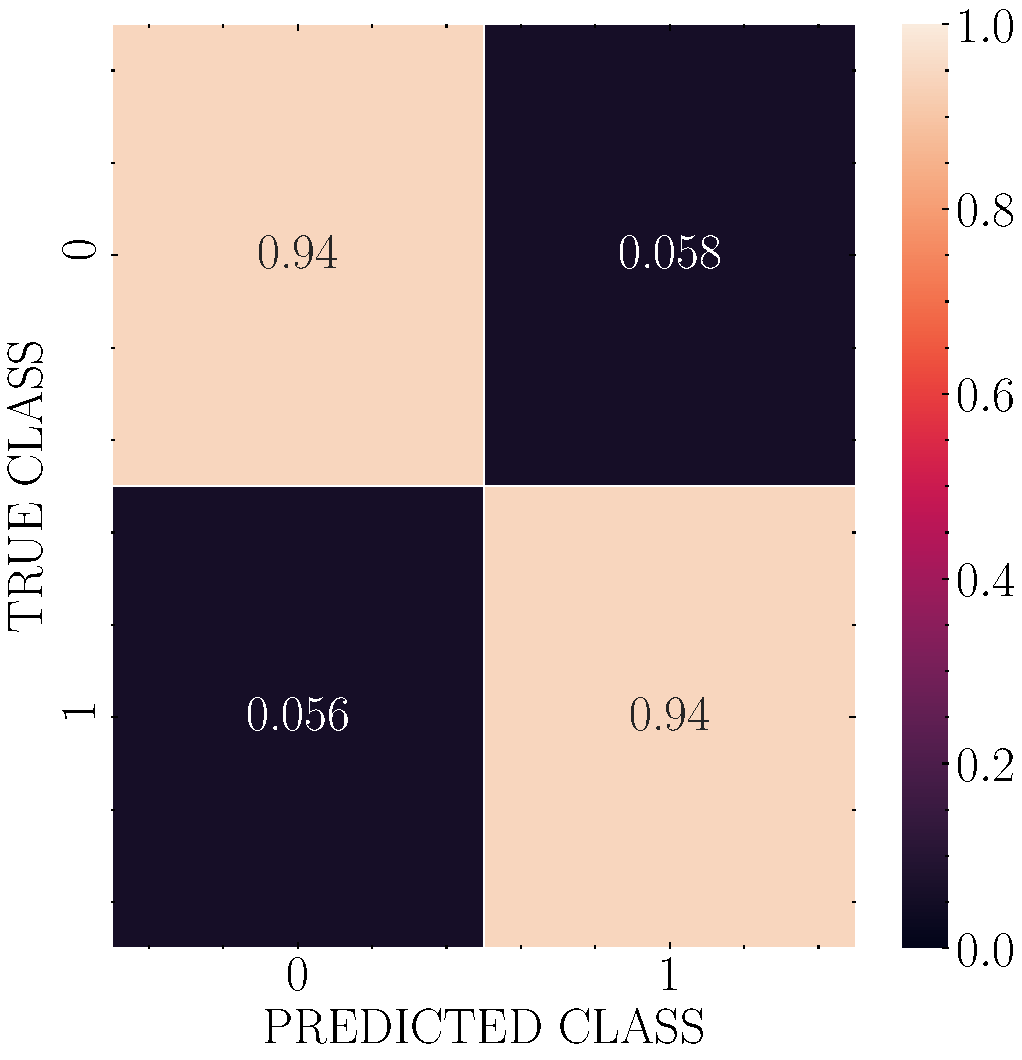
\includegraphics[width=1.5in]{../results/ex1/acc_LS_dataset_Normal_size_999.pdf}
       \caption{LS, size $999$}
       \label{fig:LS_P1a_999}
    \end{subfigure}
\quad
    \begin{subfigure}[!htbp]{0.2\textwidth}
       \centering
       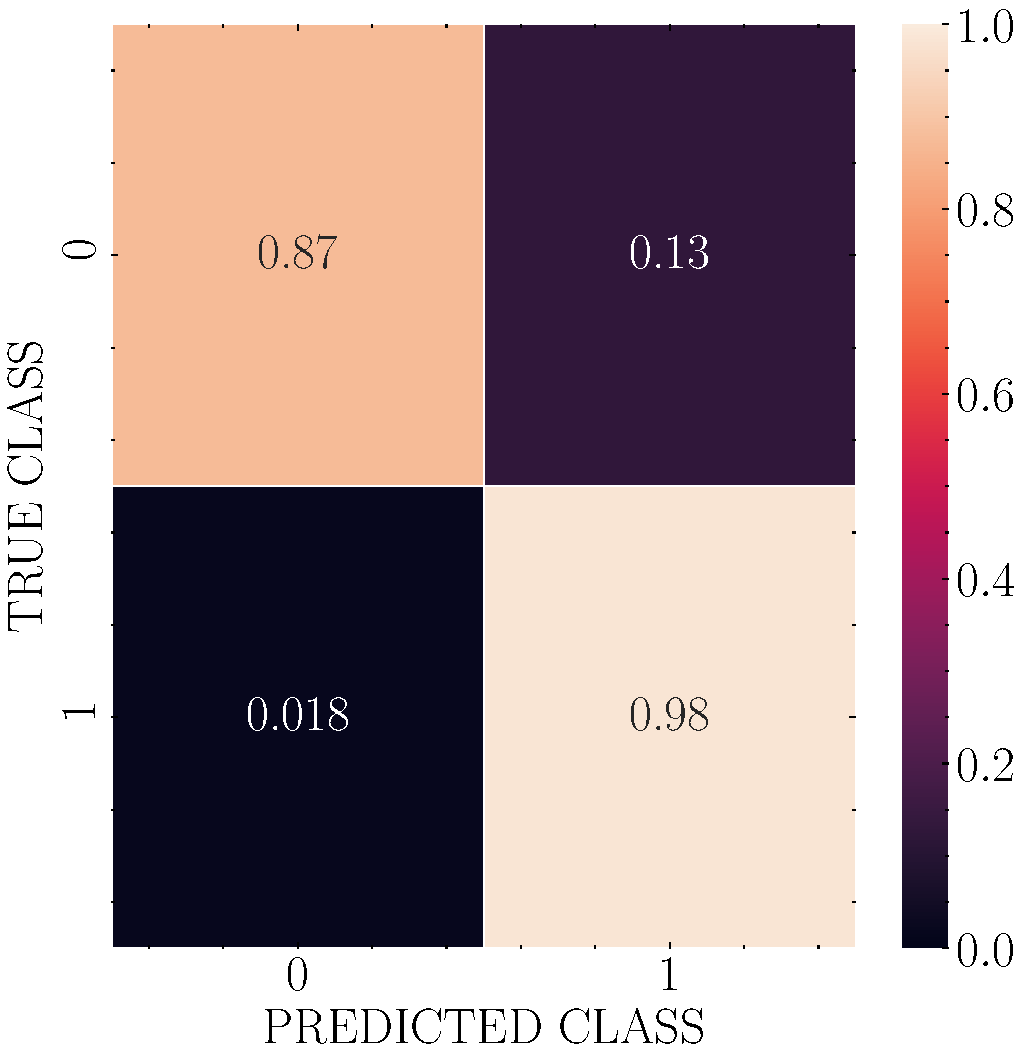
\includegraphics[width=1.5in]{../results/ex1/acc_LOG_dataset_Normal_size_999.pdf}
       \caption{LOG, size $999$}
       \label{fig:LOG_P1a_999}
    \end{subfigure}

\caption{Linear Least-Squares Classification and Logistic Regression.}
\label{fig:ex1_P1a}
\end{figure}

% ------------------------------------------------------------------------------------------------------------------------------------------------------
% ------------------------------------------------------------------------------------------------------------------------------------------------------

\section{Multi-Class Linear Model on Iris Dataset}
\label{sec:bayes20D}

\problem{Problem (2.i) One vs. Rest}
\label{prob:2.i}


% ------------------------------------------------------------------------------------------------------------------------------------------------------

\problem{Problem (2.ii) One vs. All}
\label{prob:2.ii}

% ------------------------------------------------------------------------------------------------------------------------------------------------------
% ------------------------------------------------------------------------------------------------------------------------------------------------------

\section{Logistic Regression on Financial Data}
\label{sec:german}


% ------------------------------------------------------------------------------------------------------------------------------------------------------
% ------------------------------------------------------------------------------------------------------------------------------------------------------

\section{Linear Least-Squares Regression in 1D}
\label{sec:linearRegression}


% ------------------------------------------------------------------------------------------------------------------------------------------------------
% ------------------------------------------------------------------------------------------------------------------------------------------------------

%\section{Code Repository}
%The Python codes to reproduce the results can be found in the GitHub repository \url{https://github.com/kamath-abhijith/Bayes_Classifier}. Use \texttt{requirements.txt} to install the dependencies.


\end{document} 
